%%%%%%%%%%%%%%%%%%%%%%%%%%%%%%%%%%%%%%%%%%
% Mathematics Final Year Research Projects
% LaTeX Template
% Version 1.0 (31/01/24)
%
% This template has been adapted from: https://www.overleaf.com/latex/templates/imperial-college-report-template/wncnzptkhnbc
% Students should feel free to adapt this template to their needs.
%%%%%%%%%%%%%%%%%%%%%%%%%%%%%%%%%%%%%%%%%%
%----------------------------------------------------------------------------------------
% PACKAGES AND OTHER DOCUMENT CONFIGURATIONS
%----------------------------------------------------------------------------------------
\documentclass[a4paper,11pt, titlepage]{article}

%% Language and font encodings
\usepackage[english]{babel}
\usepackage[utf8]{inputenc}
\usepackage[T1]{fontenc}
\usepackage{titlesec}
\usepackage{titletoc}
\usepackage{graphicx} % Required for inserting images
\usepackage{listings} % Required for coding
\usepackage[a4paper,top=1in,bottom=1in,left=1in,right=1in,marginparwidth=1.75cm]{geometry}
\usepackage{xcolor}
\usepackage{amsmath}
\usepackage{amssymb}
\usepackage{placeins}
\usepackage{setspace}
\usepackage{cite}
\usepackage{tikz}
\usetikzlibrary{shapes.geometric, arrows}
\usetikzlibrary{matrix}

\tikzstyle{startstop} = [rectangle, rounded corners, minimum width=3cm, minimum height=1cm,text centered, draw=black, fill=red!30]
\tikzstyle{process} = [rectangle, minimum width=3cm, minimum height=1cm, text centered, draw=black, fill=orange!30]
\tikzstyle{arrow} = [thick,->,>=stealth]
% Customizing paragraph and subparagraph to include numbering and appear in the table of contents
\titleformat{\paragraph}
  {\normalfont\normalsize\bfseries}{\theparagraph}{1em}{}
\titlespacing*{\paragraph}{0pt}{3.25ex plus 1ex minus .2ex}{1em}
\renewcommand\theparagraph{\thesubsubsection.\arabic{paragraph}}
\setcounter{secnumdepth}{4}

\titleformat{\subparagraph}
  {\normalfont\normalsize\itshape}{\thesubparagraph}{1em}{}
\titlespacing*{\subparagraph}{0pt}{3.25ex plus 1ex minus .2ex}{1em}
\renewcommand\thesubparagraph{\theparagraph.\arabic{subparagraph}}
\setcounter{secnumdepth}{5}

%% Sets page size and margins
\usepackage[a4paper,top=1in,bottom=1in,left=1in,right=1in,marginparwidth=1.75cm]{geometry}

%% Useful packages
\usepackage{afterpage}
\usepackage{amsmath}
\usepackage{amsthm}
\usepackage{amssymb}
\usepackage{csquotes}
\usepackage{enumitem}
\usepackage{graphicx}
\usepackage{subcaption}
\usepackage{lipsum}
\usepackage{booktabs}
\usepackage{url}

% Listings (for displaying code):
\usepackage{listings}
\lstset{
  basicstyle=\ttfamily,
  commentstyle=\color{gray},
  morekeywords={import, as, def, return, for, in, range, np, plt},
  frame=single,
  breaklines=true,
  postbreak=\mbox{\textcolor{red}{$\hookrightarrow$}\space},
}


% Center figure captions:
\usepackage{caption}
\captionsetup[figure]{labelfont={bf},name={Figure},labelsep=quad}
\captionsetup[table]{labelfont={bf},name={Table},labelsep=quad}

% Set no indentation for all paragraphs
\setlength{\parindent}{0pt}

% ----------- Algorithm2e setup
\usepackage[ruled,vlined]{algorithm2e}
\makeatletter
\renewcommand{\SetKwInOut}[2]{%
  \sbox\algocf@inoutbox{\KwSty{#2}\algocf@typo:}%
  \expandafter\ifx\csname InOutSizeDefined\endcsname\relax% if first time used
    \newcommand\InOutSizeDefined{}\setlength{\inoutsize}{\wd\algocf@inoutbox}%
    \sbox\algocf@inoutbox{\parbox[t]{\inoutsize}{\KwSty{#2}\algocf@typo:\hfill}~}\setlength{\inoutindent}{\wd\algocf@inoutbox}%
  \else% else keep the larger dimension
    \ifdim\wd\algocf@inoutbox>\inoutsize%
    \setlength{\inoutsize}{\wd\algocf@inoutbox}%
    \sbox\algocf@inoutbox{\parbox[t]{\inoutsize}{\KwSty{#2}\algocf@typo:\hfill}~}\setlength{\inoutindent}{\wd\algocf@inoutbox}%
    \fi%
  \fi% the dimension of the box is now defined.
  \algocf@newcommand{#1}[1]{%
    \ifthenelse{\boolean{algocf@inoutnumbered}}{\relax}{\everypar={\relax}}%
%     {\let\\\algocf@newinout\hangindent=\wd\algocf@inoutbox\hangafter=1\parbox[t]{\inoutsize}{\KwSty{#2}\algocf@typo\hfill:}~##1\par}%
    {\let\\\algocf@newinout\hangindent=\inoutindent\hangafter=1\parbox[t]{\inoutsize}{\KwSty{#2}\algocf@typo:\hfill}~##1\par}%
    \algocf@linesnumbered% reset the numbering of the lines
  }}%
\makeatother
% --------- end algorithm2e setup

% \bm allows typing bold math:
\usepackage{bm}
\usepackage[normalem]{ulem}

\usepackage[colorinlistoftodos]{todonotes}
\usepackage[colorlinks=true, allcolors=blue]{hyperref}

\renewcommand*{\rmdefault}{bch}
\renewcommand*{\ttdefault}{lmtt}
\newcommand{\citationneeded}{\textcolor{red}{[citation-needed]}}

\DeclareMathOperator*{\argmin}{\arg\!\min}
\DeclareMathOperator*{\argmax}{\arg\!\max}

% Add bigger skip between paragraphs, makes reading easier:
\setlength{\parskip}{0.5em}

% Bibliography
\usepackage[numbers, comma, square, sort&compress]{natbib}
\usepackage{natbib}
%% \bibliographystyle{abbrvunsrtnat.bst}


% Theorem, Lemma, Corollary and Proofs
\theoremstyle{definition}
\newtheorem{definition}{Definition}[section]
\theoremstyle{plain}
\newtheorem{theorem}{Theorem}[section]
\newtheorem{corollary}{Corollary}[theorem]
\newtheorem{lemma}[theorem]{Lemma}
\theoremstyle{remark}
\newtheorem*{remark}{Remark}
\theoremstyle{definition}
\newtheorem{example}{Example}

%----------------------------------------------------------------------------------------
% END OF DOCUMENT CONFIGURATION
%----------------------------------------------------------------------------------------

%----------------------------------------------------------------------------------------
% IMPORTANT INFORMATION TO MODIFY FOR THE TITLE PAGE
%----------------------------------------------------------------------------------------
\newcommand{\reporttitle}{Optimisation of Fractal Image Compression} % Title of your research project
\newcommand{\reportauthorA}{Jordan Pang (CID: 02224586)} % First Name, Last Name and CID of student 1
\newcommand{\reportauthorC}{Monique Smith (CID: 02213249)} % First Name, Last Name and CID of student 3
\newcommand{\reportauthorD}{Qixuan Mu (CID: 02284055)} % First Name, Last Name and CID of student 4
\newcommand{\reportauthorE}{Kehang Sun (CID: 02219888)} % First Name, Last Name and CID of student 5
\newcommand{\supervisor}{Jeroen S W Lamb} % First Name and Last Name of your supervisor(s)
%----------------------------------------------------------------------------------------

%----------------------------------------------------------------------------------------
% To compile this file, use the following sequence: 
%	latex main.tex
%	bibtex main.tex
%	latex main.tex
%	latex main.tex
%----------------------------------------------------------------------------------------

%----------------------------------------------------------------------------------------
% START OF DOCUMENT
%----------------------------------------------------------------------------------------
\usepackage{setspace}
\doublespacing
\usepackage{algorithm}
\usepackage{algorithmic}
\begin{document}

%%%%%%%%%%%%%%%%%%%%%%%%%%%%%%%%%%%%%
% Title page
%%%%%%%%%%%%%%%%%%%%%%%%%%%%%%%%%%%%%
\begin{titlepage}
\newcommand{\HRule}{\rule{\linewidth}{0.5mm}} % Defines a new command for the horizontal lines, change thickness here
%----------------------------------------------------------------------------------------
%	LOGO SECTION
%----------------------------------------------------------------------------------------

\includegraphics[width=8cm]{Imperial_logo.png}\\[1cm] % Include a department/university logo - this will require the graphicx package
%----------------------------------------------------------------------------------------
\center % Center everything on the page
%----------------------------------------------------------------------------------------
%	HEADING SECTIONS
%----------------------------------------------------------------------------------------
% For M3R or M4R reports, comment out as appropriate
\textsc{\LARGE Imperial College London}\\[0.5cm] 
\textsc{\Large Department of Mathematics}\\[1.5cm] 
\textsc{\Large Second-year Group Research Project}\\[0.5cm]
%----------------------------------------------------------------------------------------
%	TITLE SECTION
%----------------------------------------------------------------------------------------
\makeatletter
\HRule \\[0.6cm]
{ \huge \bfseries \reporttitle}\\[0.6cm] % Title of your document
\HRule \\[1.5cm]
%----------------------------------------------------------------------------------------
%	AUTHOR SECTION
%----------------------------------------------------------------------------------------
\begin{minipage}{0.4\textwidth}
\begin{flushleft} \large
\emph{Author:}\\
\reportauthorA \\
\reportauthorB \\
\reportauthorC \\
\reportauthorD \\
\reportauthorE
\end{flushleft}
\end{minipage}
~
\begin{minipage}{0.4\textwidth}
\begin{flushright} \large
\emph{Supervisor(s):} \\
\supervisor % Supervisor's name
\end{flushright}
\end{minipage}\\[2cm]
\makeatother
%----------------------------------------------------------------------------------------
%	FOOTER & DATE SECTION
%----------------------------------------------------------------------------------------
\vfill
\makeatletter
{\large \today}\\[2cm] % Date, change the \today to a set date if you want to be precise
\makeatother
\end{titlepage}
%%%%%%%%%%%%%%%%%%%%%%%%%%%%%%%%%%%%%

%%%%%%%%%%%%%%%%%%%%%%%%%%%%%%%%%%%%%
% Abstract
\begin{abstract}
Fractal image compression (FIC) exploits the self-similar properties of images to achieve high compression ratios, making it an efficient technique for storing and transmitting images. The main goal of this project is to develop a program that takes an image as an input and approximate any self-similar properties into contraction mappings so that we can reconstruct the fractal image by iteration.

Our ideas predominantly stem from the Banach Fixed-Point Theorem and the Collage Theorem, which allow us to approximate a set \( B \) by compiling a finite number of contractive copies of \( B \) constructed by \( f_i(B) \). Specifically, if we have a collection of contraction mappings \( F = \{ f_i : i \in I \} \), then the attractor \( A \) of \( F \), the unique fixed point, is very similar to \( B \).

In this way, we can, in a sense, obtain a formula for a set \( B \), and this approach is essential in image compression. By representing an image as a set \( B \), we can use the attractor \( A \) to achieve efficient and accurate compression.

Along the way, we present two different algorithms of generating a fractal image: The Deterministic Algorithm and The Random Iteration Algorithm. The Deterministic Algorithm applies all transformations to the entire image iteratively, which can computationally intensive and time-consuming, especially for higher-resolution images and complex transformation sets. In contrast, The Random Iteration Algorithm applies randomly selected transformations to randomly chosen points, supplying a probabilistic approach that often converges faster and requires less computational effort.

Finally, we explore the Inverse IFS problem - to find a set of affine transformations from a given image as the attractor. To tackle this, we researched into the fields of machine learning and applied optimisation techniques such as K-Means Clustering and Gradient Descent algorithms to enhance the compression process.

\end{abstract}
%%%%%%%%%%%%%%%%%%%%%%%%%%%%%%%%%%%%%
 
%%%%%%%%%%%%%%%%%%%%%%%%%%%%%%%%%%%%%
% Table of contents
\tableofcontents
\clearpage
%%%%%%%%%%%%%%%%%%%%%%%%%%%%%%%%%%%%%

%%%%%%%%%%%%%%%%%%%%%%%%%%%%%%%%%%%%%
% Main sections
%%%%%%%%%%%%%%%%%%%%%%%%%%%%%%%%%%%%%
\section{Introduction to Fractal Image Compression (FIC)}
\label{sec:introduction}

\subsection{Overview of Fractal Image Compression (FIC)}
Fractal Image Compression(FIC) is a method of compressing digital images using the mathematical principles of fractals. This approach is considered lossy, meaning some data is lost during compression. It is effective in specific scenarios, particularly with images of natural scenes and textures. Fractal algorithms convert the similar parts of the natural image into “fractal code”, which can be used to recreate the image.\cite{may1996fractal}

\subsection{Definition of Fractal}
In 1918, Felix Hausdorff introduced a notion of "fractional dimension", which is a property held by complex geometrical figures known as fractals. Fractals are intricate geometric shapes that display self-similarity across various scales. This indicates that a fractal shape can be broken down into smaller segments, each of which is a scaled-down version of the entire shape. Fractals are found both in natural environments and in mathematical frameworks, and they are distinguished by their complex patterns and endless details. They are capable of depicting various irregular shapes and spatially uneven features in nature, including mountain ranges and coastlines.\cite{britannica_fractal}

\subsection{Key Property of Fractals}
\begin{itemize}
    \item \textbf{Self-Similarity}
    \begin{itemize}
        \item The self-similarity is a property of objects or patterns where a part of the structure resembles the whole structure. This means that if you take a small section of a self-similar object and magnify it, the magnified section will look similar to the larger object. This characteristic can be found both in nature and in mathematical constructs.
    \end{itemize}
    \item \textbf{Fractal Dimension}
    \begin{itemize}
        \item Unlike the Euclidean dimension, the fractal dimension is a parameter, typically represented by a non-integer, meaning it represents a fraction rather than an integer.
        \item Traditional geometry uses integer dimensions: a line is one dimensional, a plane is two dimensional, and a solid object is three dimensional. However, fractal dimensions are often non-integer values, indicating a complexity that falls between these standard dimensions. The main formula used to calculate the fractal dimension of a fractal is $r^D = n$, where $r$ is a scaling factor, $D$ is fractal dimension and $n$ is the number of pieces after one division of the shape.
    \end{itemize}
    \item \textbf{Infinite Complexity}
    \begin{itemize}
        \item Fractals have infinite detail, meaning that as you magnify into a fractal, new patterns and structures continue to emerge. This is why fractals are often described as infinitely complex.
    \end{itemize}
    \item \textbf{Generation by Iterative Processes}
    \begin{itemize}
        \item Many fractals are generated using iterative processes, where a simple initial shape is repeatedly transformed by a set of rules. And this iterative process is IFS, which can be employed to create fractal images.
    \end{itemize}
    
\end{itemize}


\subsection{Iterated Function System (IFS)}
Iterated Function System is a mathematical framework used to construct fractals, which are complex geometric shapes characterized by self-similarity and intricate patterns. IFS employs a set of contraction mappings to generate fractals through an iterative process.
Here are some examples of Fractals, with their IFS:
\begin{itemize}
    \item \textbf{The Barnsley Fern} is perhaps the most famous example of an IFS in nature. This fractal mimics the structure of a natural fern, with each leaf segment appearing as a smaller copy of the whole. Michael Barnsley used an IFS to create a mathematical representation of a fern, demonstrating how simple recursive formulas can mimic complex natural shapes.
    \begin{figure}[h]
    \centering
    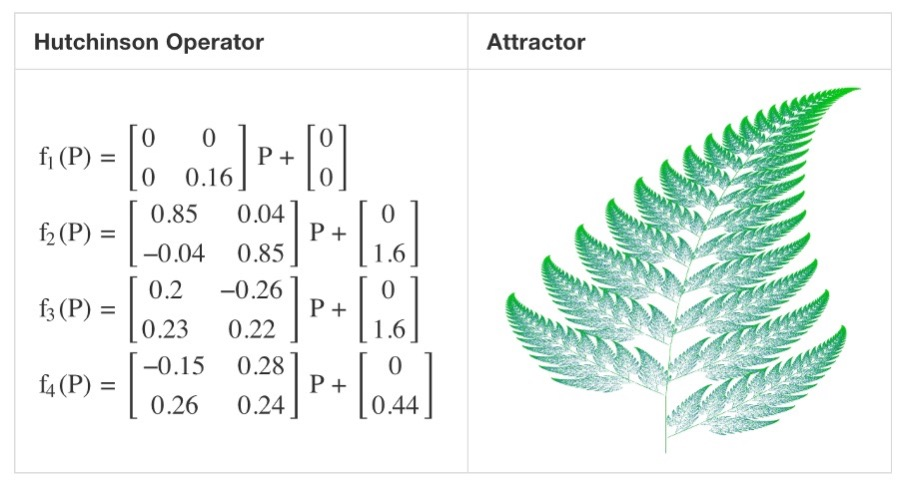
\includegraphics[width=0.8\textwidth]{pic1.jpg}
    \caption{Hutchinson Operator and Attractor of Barnsley Fern\cite{algorithmarchive2024IFS}}
    \label{fig:BarnsleyFern}
    \end{figure}

    \item \textbf{Trees and Plants} often exhibit fractal-like branching patterns where branches and even sub-branches form self-similar structures. This recursive pattern can be modeled using IFS, where each transformation in the system represents a different type of branching or growth direction.
    \begin{figure}[h]
    \centering
    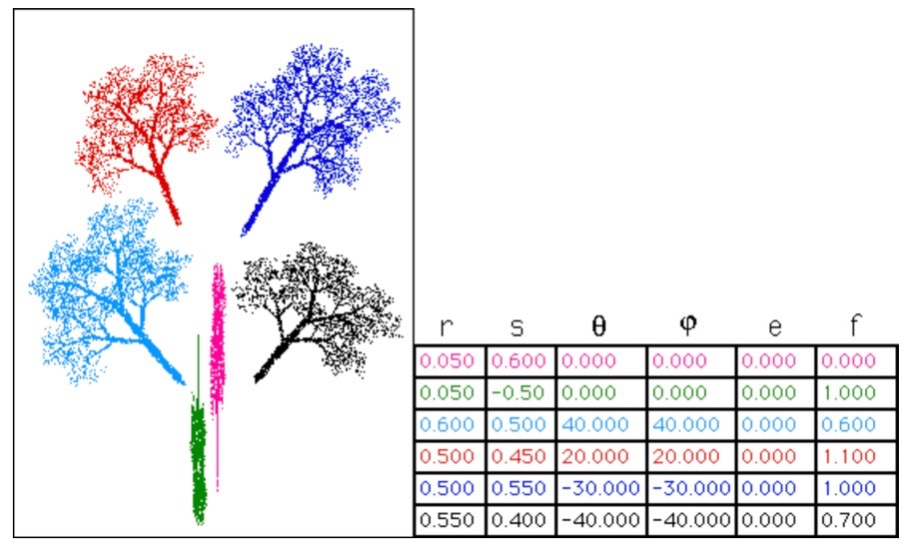
\includegraphics[width=0.8\textwidth]{pic2.jpg}
    \caption{IFS of tree\cite{treeIFS}}
    \label{fig:BarnsleyFern}
    \end{figure}
\end{itemize}

\subsection{Affine Transformation}
\begin{figure}[ht]
    \centering
    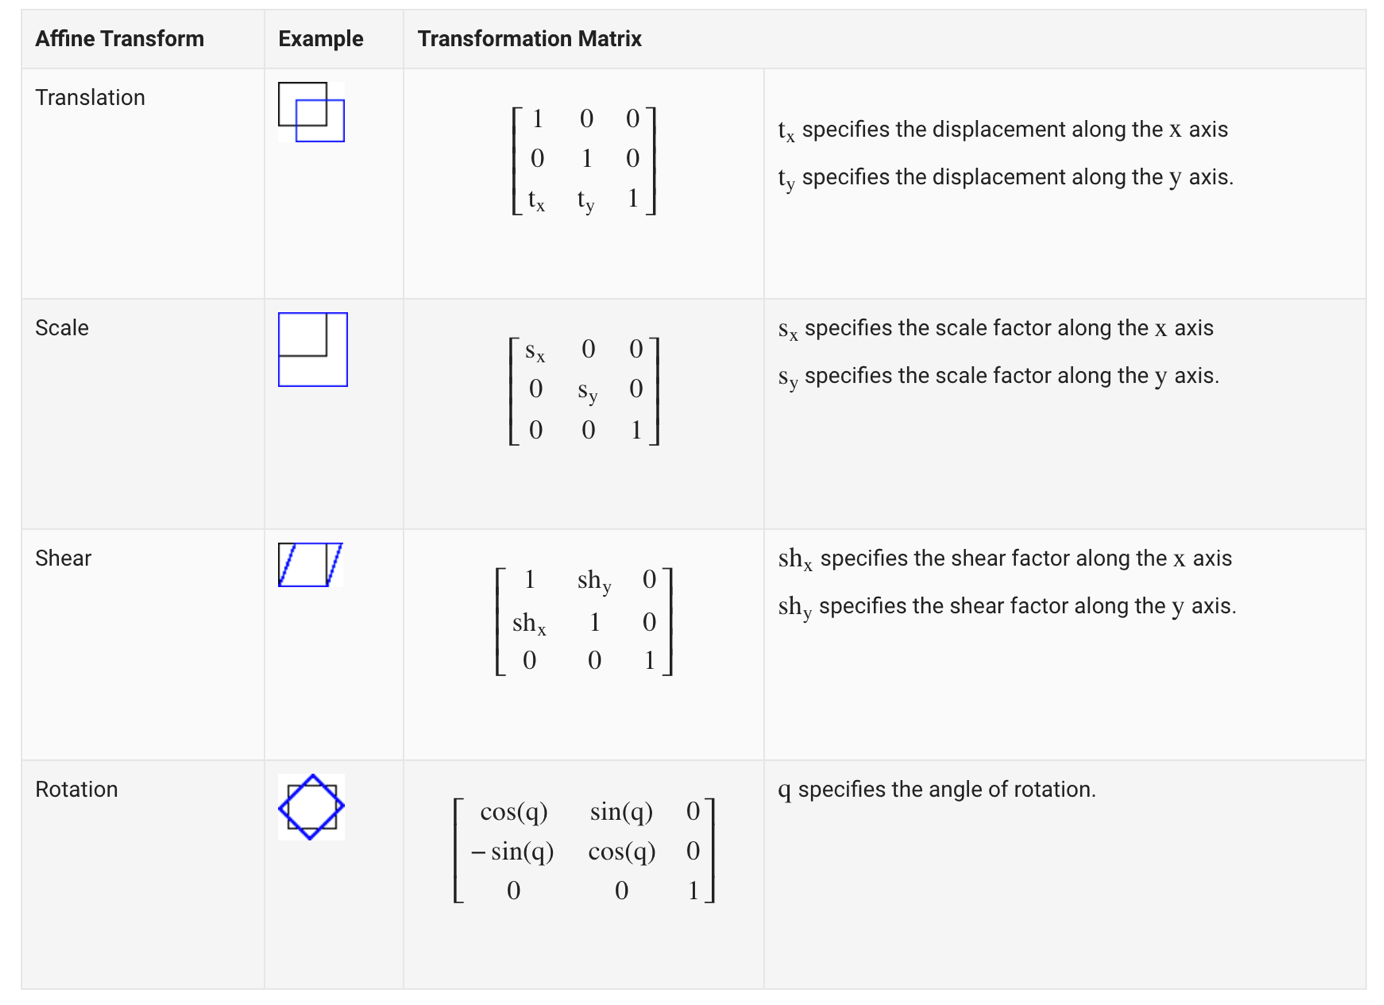
\includegraphics[width=0.9\linewidth]{pic4.png}
    \caption{Affine transformation\cite{mathworksTransformations}}
    \label{fig:pic4}
\end{figure}
An affine transformation is a type of linear transformation that encompasses translation, scaling, shearing, and rotation. It preserves the straightness and parallelism of objects. Affine transformation matrices enable various geometric operations on images. In fractal image compression, affine transformations are used to map source blocks to destination blocks to find the best match and achieve compression. 

\section{Theorem and Proofs}
\subsection{Fractal Metric Space and Some basic properties}
To study fractal geometry, we must first introduce the space in which fractals exist.
\begin{definition}
Given a complete metric space $(\mathbf{X}, d)$, $\mathcal{H}(\mathbf{X})$ is the space consisting of all non-empty compact subsets of $\mathbf{X}$.
\end{definition}

Naturally, we provide the definition of the distance from a point, $x \in \mathbf{X}$, to a set $B$ in $\mathcal{H}(\mathbf{X})$.

\begin{definition}
Suppose $(\mathbf{X}, d)$ is a complete metric space, $x \in \mathbf{X}$, and $B \in \mathcal{H}(\mathbf{X})$. We define the distance from $x$ to $B$ as
\[
d(x, B) = \min\{d(x, y) : y \in B\}.
\]
This $d(x, B)$ represents the minimum distance from the point $x$ to any point in the set $B$.
\end{definition}

Similarly, we can define the distance between two sets, $A, B \in \mathcal{H}(\mathbf{X})$.
\begin{definition}
Suppose $(\mathbf{X}, d)$ is a complete metric space, and let $A, B \in \mathcal{H}(\mathbf{X})$. We define the distance between sets $A$ and $B$ as
\[d(A, B) = \max\{d(x, B) : x \in A\}.\]
Here, $d(A, B)$ denotes the distance from the set $A$ to the set $B$ within the space $\mathcal{H}(\mathbf{X})$.
\end{definition}

\begin{remark}
It is obvious that the minimum and maximum can be attained. Let's examine a function \( f: B \rightarrow \mathbb{R} \) defined by
\[
f(y) = d(x, y) \quad \text{for all } y \in B.
\]
This function is clearly continuous in $(B, d)$. At the same time, $(B, d)$ is a compact metric space from the way $\mathcal{H}(X)$ is chosen. By the Extreme Value Theorem, $f$ can attain its minimum. Similar reasoning implies a maximum can be attained. Now we define the Hausdorff distance.
\end{remark}

\begin{definition}{(Hausdorff distance).}
Suppose $(\mathbf{X}, d)$ is a complete metric space. For $A, B \in \mathcal{H}(\mathbf{X})$, the Hausdorff distance is defined as
\[
h(A, B) = \max(d(B, A), d(A, B))= d(A, B) \lor d(B, A).
\]
\end{definition}
\begin{remark}
By observing the structure of the Hausdorff distance, it is very sensitive to any outliers and this point may only occupy a small part of the overall image.
\end{remark}

The Hausdorff distance is indeed a metric. One can easily verify the three properties of positivity, symmetry and the triangle inequality.

Next, we briefly introduce an important definition that will aid us in our gradient descent program for the Inverse IFS problem, as an alternative more efficient distance metric.

\begin{definition}{(Chamfer distance).}
For $A, B \in \mathcal{H}(\mathbf{X})$, the Chamfer distance is defined as
\[
d_C(A, B) = \sum_{a \in A} \min_{b \in B} \| a - b \|^2 + \sum_{b \in B} \min_{a \in A} \| b - a \|^2
\]
\end{definition}

\begin{theorem}
Suppose $(X, d)$ is a complete metric space. Then $(\mathcal{H}(X), h)$ is also a complete metric space. Furthermore, if $\{A_k \in \mathcal{H}(X)\}_{k=1}^{\infty}$ is a Cauchy sequence, then
\[
A = \lim_{k \to \infty} A_k \in \mathcal{H}(X)
\]
can be characterized as follows:
\[
A = \{a \in X : \text{there exists a Cauchy sequence } \{a_k \in A_k\} \text{ such that } a_k \to a\}.
\]
\end{theorem}
Proving completeness is equivalent to showing that every Cauchy sequence converges in the space. Specifically, there are three points to guide one through such proof:

\begin{enumerate}
    \item Existence of a limit.
    \item The limit is within the space (the limit is compact, i.e., the limit is closed and totally bounded).
    \item This limit is of the chosen Cauchy sequence.
\end{enumerate}

Before we delve into the main theorems of our project, we take a moment to compare and analyse the efficiency of distance metrics that we use in the rest of our report.

\begin{remark}
Choosing an appropriate efficient distance metric is essential in ensuring accurate image compression, by means of deducing the degree of similarity between the target image and the image produced by iterating a set of transformations. In terms of time complexity, the Hausdorff distance and Chamfer distance both follow the same overall time complexity of $O(n^2)$. To see this, consider two sets $A, B$, each consisting of $n$ points. In both distance functions, $\forall a \in A$, we find the closest point in $B$, thus giving $n^2$ distance calculations. The difference lies in how the $n^2$ calculations are treated - the Hausdorff metric records maximum distances, which can be very computational heavy, whereas the Chamfer distance focuses on averages, which is practically preferable since it is less sensitive to outliers and more manageable to implement. However, there are disadvantages to using the Chamfer distance, for example, the distances may be underestimated when points are sparse. Clearly, an optimal distance metric for efficient image compression is very challenging to discover. Examples, not discussed in the report include: Structural Similarity Index Measure (SSIM), Mean Squared Error (MSE), Earth Mover's Distance (EMD). We discuss one briefly - SSIM - returning a value $x, -1 \leq x \leq 1$, measuring the structural (brightness, contrast, etc) similarity between two 'patches' of pixels. It correlates nicely with human visual perception, but the formulae are very complex, involving mean, variance covariance values of 'patches'.
\end{remark}

\subsection{Iterated Function System and Collage Theorem}

In the next part of the chapter, we will introduce the essence of contractive mappings in relation to iterated function systems and how this naturally leads to the construction of the Collage theorem.

\begin{definition}
Let \( X \) be a metric space with a metric \( d \). A function \( f : X \to X \) is called Lipschitz continuous with Lipschitz constant \( a \) if there exists \( a \in \mathbb{R}_{>0} \) such that
\[
d(f(x), f(y)) \leq a \cdot d(x, y) \quad \forall x, y \in X.
\]
If the Lipschitz constant \( a \) is less than 1, then \( f \) is termed \textit{contractive} with contractivity \( a \).
\end{definition}

\begin{definition}{(IFS). }
Suppose \( X \) is a complete metric space. An iterated function system consists of a collection of contractive maps \( f_k : X \to X \) for \( k = 1, \ldots, n \).
\end{definition}

\begin{lemma}
Consider a contraction mapping \( f : X \to X \) on the metric space \( (X, d) \) with a contractivity factor \( a \). Define the mapping \( f : \mathcal{H}(X) \to \mathcal{H}(X) \) by
\[
f(A) = \{ f(x) : x \in A \} \quad \forall A \in \mathcal{H}(X).
\]
This map \( f \) is a contraction on the metric space \( (\mathcal{H}(X), h(d)) \) with the same contractivity factor \( a \).
\end{lemma}

The next lemma is vital in allowing us to determine IFS of a fractal, making a union of contraction mappings a contraction.

\begin{lemma}
Let \((X, d)\) be a metric space. Consider the set of contraction mappings \(\{f_k : k = 1, 2, \ldots, n\}\) on \((\mathcal{H}(X), h)\), where each \(f_k\) has a contractivity factor \(a_k\). Define \(W : \mathcal{H}(X) \to \mathcal{H}(X)\) by
$$
W(A) = \bigcup_{k=1}^n f_k(A),
$$
for each \(A \in \mathcal{H}(X)\).

Then \(W\) is a contraction mapping with contractivity factor \(a = \max \{a_k : k = 1, 2, \ldots, n\}\).
\end{lemma}

Naturally, this leads to the construction of the following theorem.

\begin{theorem}
Let \(\{X; f_k, k = 1, 2, \ldots, n\}\) be an iterated function system with a contractivity factor \(a\). Define the map \(W : \mathcal{H}(X) \to \mathcal{H}(X)\) by
$$
W(A) = \bigcup_{k=1}^n f_k(A)
$$
for all \(A \in \mathcal{H}(X)\). This map \(W\) is a contraction mapping on the complete metric space \((\mathcal{H}(X), h(d))\) with contractivity factor \(a\). Specifically,
$$
h(W(A), W(B)) \leq a \cdot h(A, B)
$$
for all \(A, B \in \mathcal{H}(X)\). The unique fixed point \(C \in \mathcal{H}(X)\) satisfies
$$
C = W(C) = \bigcup_{k=1}^n f_k(C)
$$
and is given by
$$
C = \lim_{m \to \infty} W^m(A)
$$
for any \(A \in \mathcal{H}(X)\). This fixed point \(C \) is called the \textit{attractor} of the IFS.

\end{theorem}

Here we had made use of the following theorem:

\begin{theorem}[The Banach Fixed-Point Theorem]
Suppose \(X\) is a complete metric space and \(f : X \to X\) is a contraction mapping. Then there exists a unique point \(x_f \in X\) such that for any \(x \in X\),
$$
x_f = f(x_f) = \lim_{n \to \infty} f^{\circ n}(x).
$$
This point is known as the fixed point or attractor of the mapping \(f\). Furthermore,
$$
d(x, x_f) \leq \frac{d(x, f(x))}{1 - a} \quad \forall x \in X.
$$

\end{theorem}
Applying this theorem to this metric space$(\mathcal{H}(X), h)$, we attain the Collage Theorem:



\begin{theorem}[The Collage Theorem]
Suppose \((X, d)\) is a complete metric space and \(L \in \mathcal{H}(X)\) is given, along with \(\epsilon \geq 0\). Select an IFS \(\{X; (f_1, f_2, \ldots, f_k)\}\) with contractivity factor \(0 \leq a < 1\), such that
$$
h(L, \bigcup_{k=1}^n f_k(L)) \leq \epsilon,
$$
where \(h(d)\) denotes the Hausdorff metric. Then,
$$
h(L, A) \leq \frac{\epsilon}{1 - a},
$$
where \(A\) is the attractor of the IFS. Alternatively,
$$
h(L, A) \leq \frac{h(L, \bigcup_{k=1}^n f_k(L))}{1 - a}
$$
for any \(L \in \mathcal{H}(X)\).
\end{theorem}

The above theorem is very useful in finding the related Iterated Function Systems (IFS). It gives us a method to control the initial difference of a given set under suitable affine maps. As a result, we can control the difference between the attractor and the initial given set. This theorem provides the basis for solving the fractal inverse problem and for fractal image compression. It simplifies the problem of attractor generation from an iterative process to solely comparing the attractor with a single iteration of the IFS.



\section{Two algorithms}

The algorithms discussed include the Deterministic Algorithm and the Random Iteration Algorithm. Deterministic Algorithm uses a fixed sequence of transformations to directly generate the fractal, while the Random Iteration Algorithm relies on stochastic selection to approximate the fractal attractor over many iterations.

\subsection{The Deterministic Algorithm \cite{barnsley2014fractals}}

Let $\{X; f_1, f_2, \ldots, f_N\}$ be an IFS. Select a compact set $A_0 \subset \mathbb{R}^2$. Then compute successively $A_k = W^{n}(A)$ according to
\[
A_{k+1} = \bigcup_{j=1}^k f_j(A_k) \quad \text{for} \, k = 1, 2, \ldots
\]

Thus construct a sequence $\{A_k : k = 0, 1, 2, \ldots\} \subset \mathcal{H}(X)$. Then, by an application of Elton's Theorem (discussed later), the sequence $\{A_k\}$ converges to the attractor of the IFS in the Hausdorff metric.

So the steps of the algorithm is:

\begin{enumerate}
    \item \textbf{Initial Set}: Choose an initial compact set \( A_0 \subset \mathbb{R}^2 \).
    \item \textbf{Affine Transformations}: Define a set of affine transformations \( \{f_1, f_2, \ldots, f_N\} \), which have contraction properties.
    \item \textbf{Iteration}: Compute the successive sets \( A_{n+1} \) as the union of the transformed sets:
    \[
    A_{n+1} = \bigcup_{j=1}^N w_j(A_n)
    \]
    \item \textbf{Convergence}: Continue iterating until the sequence \( \{A_n\} \) converges to the attractor in the Hausdorff metric, according to the theory of fractals.
\end{enumerate}

Here is some pseudocode for a deterministic algorithm:

\begin{algorithm}
\caption{Pseudocode for the Deterministic Algorithm}
\begin{algorithmic}[1]
    \STATE Define affine transformations \(w_1, w_2, w_3, w_4\)\;
    \STATE Initialize points with \((0, 0)\)\;
    \FOR{each iteration} 
        \FOR{each transformation  \(w_i\)}
        \STATE Apply \(w_i\) to \((x, y)\) to get \((x', y')\)\;
            Add \((x', y')\) to new\_points\;
        \ENDFOR
    \ENDFOR
    \STATE Plot points\;
\end{algorithmic}
\end{algorithm}


\begin{figure}[h]
    \centering
    \begin{subfigure}[b]{0.45\textwidth}
        \centering
        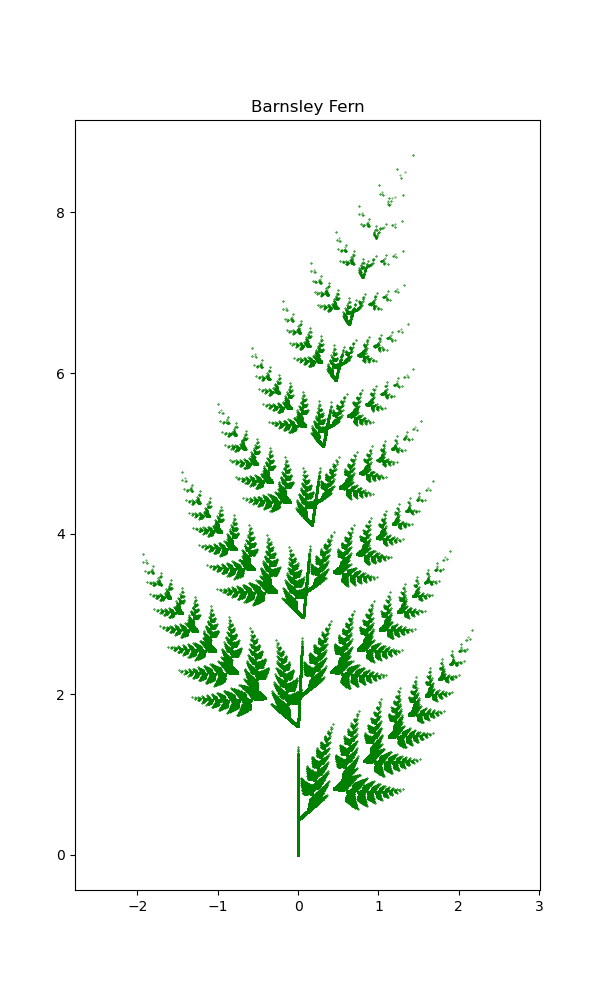
\includegraphics[width=\textwidth]{barnsley_fern_deterministic.png}
        \caption{Barnsley Fern (Deterministic)}
        \label{fig:fern_deterministic}
    \end{subfigure}
    \hfill
    \begin{subfigure}[b]{0.45\textwidth}
        \centering
        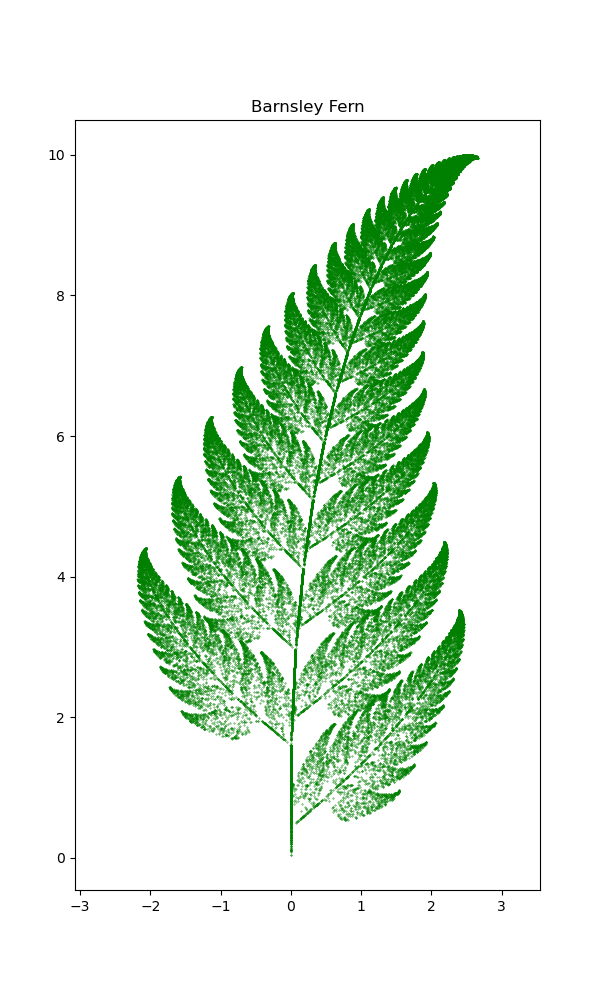
\includegraphics[width=\textwidth]{barnsley_fern_random.png}
        \caption{Barnsley Fern (Random Iteration)}
        \label{fig:fern_random}
    \end{subfigure}
    \caption{Barnsley Fern generated by Deterministic and Random Iteration Algorithms}
    \label{fig:fern_comparison}
\end{figure}

\begin{remark}
    The Deterministic Algorithm for fractal generation is computationally intensive and time-consuming because it applies all transformations to every point in each iteration, leading to rapid growth in point numbers and high memory usage. This approach often recalculates many redundant points, making it inefficient and slower to converge to the fractal attractor.
\end{remark}

Figure \ref{fig:fern_comparison} shows a Barnsley Fern generated by deterministic algorithm and random iteration algorithm (which we discuss later).

\subsubsection{Lindenmayer Systems (L-systems)}
One application of the determinstic algorithm is the L-system. Originally devised in 1968 by biologist Aristid Lindenmayer, L-systems are one fascinating method to generate fractal images algorithmically. Informally, this method is centralised around re-writing, where we select a part of an initial geometrical object and iteratively replace that part until we reach the fixed attractor in fractal terms. Now, we propose the following definition:

\begin{definition}
(L-system)\cite{lok2017educationmath}. An L-system consists of a set of alphabetical symbols
\[
X = \{x_{1}, x_{2}, ..., x_{n}\}, \quad n \in \mathbb{N},
\]
along with a production map
\[ P : X \to Y \]
\[ x \mapsto P(x), \]
where \( Y \) is the collection of strings formed by symbols from \( X \), and an axiom (initial string)
\[ x^{(0)} \in Y\]
\end{definition}

In practice, we can input several production rules for our production map and number of times to iterate the rewriting operations from the beginning axiom to produce the string of symbols that we would like. Before providing some examples, there are several types of L-systems that we can create, such as deterministic, context-free, and context-sensitive, stochastic. A deterministic L-system has only one production rule per symbol, i.e. \(\forall x \in X, \exists P(x) \in Y\). A context-free L-system applies production rules per symbol without considering the neighbouring symbols. Whereas, in a context-sensitive L-system, production rules do depend on the neighbouring symbols. Finally in a stochastic L-system, each symbol may have multiple production rules, each with an associated probability.

\begin{example}
An example of a deterministic, context-free L-systems (D0L-systems) is: 

\begin{itemize}[label={}, left=0pt]
    \item \textbf{Alphabet}: \(\quad V = \{F, \ G, \ +, \ -\}\)
    \item \textbf{Axiom (initial string)}: \(\quad F\)
    \item \textbf{Production rules}: \(F \rightarrow F + G \quad, \quad G \rightarrow F - G\)

\end{itemize}

In an L-system, there is typically an underlying interpretation for each variable/constant in the alphabet. In this case, \( F \) represents "move ahead", \( + \) means "rotate anti-clockwise \(\alpha^\circ\)", and \( - \) means "rotate clockwise \(\alpha^\circ\)", where \(\alpha\) \(\in\) \(\mathbb{R}\) . If we work through the stages of this L-system, iterating the initial axiom, we get:


\begin{itemize}[label={}, left=0pt, align=left, itemsep=0pt, parsep=0pt, topsep=0pt]
    \item \textbf{Axiom}: \(\quad F\)
    \item \textbf{Stage 1}: \(\quad F+G\)
    \item \textbf{Stage 2}: \(\quad F+G+F-G\)
    \item \textbf{Stage 3}: \(\quad F+G+F-G+F+G-F-G\)
    \item \textbf{Stage 4}: \(\quad F+G+F-G+F+G-F-G+F+G+F-G-F-G+F-G\)
\end{itemize}
\end{example}

As a result, by continuing the stages iteratively, we get gain closer and closer to the well-known Dragon Curve. This may not seem clear in terms of string rewriting, however if we take the string from the final stage of our iteration, we can interpret it visually through a geometrical object in python.\\
We implement this through turtle graphics below, showing vital parts of the code. In Algorithm 2, we have a turtle starting at $(0,0)$, facing north, taking in a string of instructions to follow. Reading each character, we draw a line through a sequence of coordinates. In this case, any uppercase letter A-J will move the turtle forward, drawing a line, and any lowercase letter a-j will move the turtle forward skipping a line. This allows more combinations of rewriting sequences. '[' records the current location of the turtle, while ']' teleports back to the location recorded by the corresponding '['.

\begin{algorithm}
\caption{Pseudocode for the construction of the Dragon Curve using L-systems \cite{butlerLSys}}
\begin{algorithmic}[1]
\REQUIRE turtle\_instructions, rotate\_amount=45
\STATE saved\_states\_after\_branching $\leftarrow$ list()
\STATE initial\_state $\leftarrow$ (0.0, 0.0, 90.0)
\STATE yield (0, 0)
\FOR{instruction in turtle\_instructions}
    \STATE $(x, y, angle) \gets \text{current\_state}$
    \IF{instruction in 'abcdefghij'}
        \STATE $\text{current\_state} \gets (x - \cos(\text{radians}(angle)), y + \sin(\text{radians}(angle)), angle)$
        \IF{instruction.islower()}
            \STATE \textbf{yield} $(\text{float('nan')}, \text{float('nan')})$
        \ENDIF
        \STATE \textbf{yield} $(\text{current\_state}[0], \text{current\_state}[1])$
    \ENDIF
    \IF{instruction == '+'}
        \STATE $\text{current\_state} \gets (x, y, angle + \text{rotate\_amount})$
    \ELSIF{instruction == '-'}
        \STATE $\text{current\_state} \gets (x, y, angle - \text{rotate\_amount})$
    \ELSIF{instruction == '['}
        \STATE $\text{saved\_states\_after\_branching.append(current\_state)}$
    \ELSIF{instruction == ']'}
        \STATE $\text{current\_state} \gets \text{saved\_states\_after\_branching.pop()}$
        \STATE \textbf{yield} $(\text{float('nan')}, \text{float('nan')})$
        \STATE $x, y, \_ \gets \text{current\_state}$
        \STATE \textbf{yield} $(x, y)$
    \ENDIF
\ENDFOR
\end{algorithmic}
\end{algorithm}


Now, we are able to convert turtle instructions to a list of coordinates which we need in order to plot the turtle movement on a graph. Then we utilise \textit{turtle\_to\_coordinates}, the function in Algorithm 2, to plot L-system sequences on a graph, given a number of iterations.

\begin{algorithm}
\caption{Pseudocode for generating a fractal plot using L-systems \cite{butlerLSys}}
\begin{algorithmic}[1]
\REQUIRE initial\_string, production\_rules, iterations=0, rotate\_amount=45
\STATE turtle\_instructions $\gets$ transform\_multiple(initial\_string, production\_rules, iterations) \textcolor{gray}{// Iterates the transformation 'iterations' number of times}
\STATE plot\_coordinates(turtle\_to\_coordinates(turtle\_instructions, rotate\_amount)) \textcolor{gray}{// Convert the instructions into a graph plot}
\end{algorithmic}
\end{algorithm}

To conclude, we present examples of what the function can produce: (a) Dragon Curve: \textit{final\_plot('FX', \{'X': 'X+YF+', 'Y': '-FX-Y'\}, 11, 90)}, (b) Shrub: \textit{final\_plot('X', \{'X': 'F-[[X]+X]+F[+FX]-X', 'F': 'FF'\}, 5, 22.5)}.

\begin{figure}[h]
    \centering
    \begin{subfigure}[b]{0.48\textwidth}
        \centering
        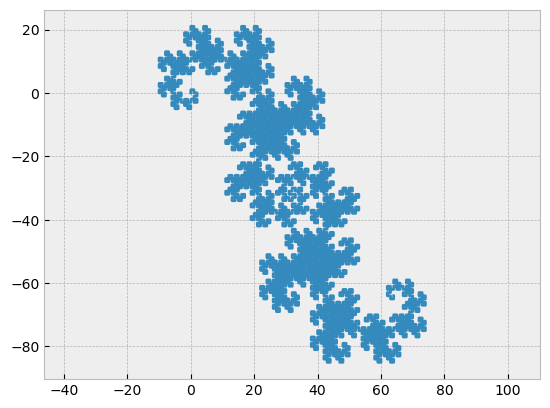
\includegraphics[width=\textwidth]{pic5.png}
        \caption{Dragon Curve}
        \label{fig:image1}
    \end{subfigure}%
    \hfill
    \begin{subfigure}[b]{0.48\textwidth}
        \centering
        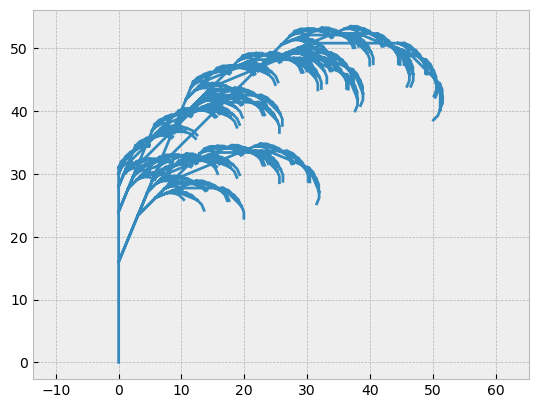
\includegraphics[width=\textwidth]{pic6.png}
        \caption{Shrub}
        \label{fig:image2}
    \end{subfigure}
    \caption{Fractal plots using L-systems}
    \label{fig:main}
\end{figure}




\subsection{The Random Iteration Algorithm}

Let $\{X; f_1, f_2, \ldots, f_N\}$ be an IFS, where probability $p_k > 0$ has been assigned to $f_k$ for $k = 1, 2, \ldots, N$, where $\sum_{k=1}^N p_k = 1$. Choose $x_0 \in X$ and then choose recursively, independently,
\[
f_n \in \{f_1(x_{n-1}), f_2(x_{n-1}), \ldots, f_N(x_{n-1})\} \quad \text{for} \; n = 1, 2, 3, \ldots,
\]
where the probability of the event $x_n = w_k(x_{n-1})$ is $p_k$. Thus, construct a sequence $\{x_k : k = 0, 1, 2 \ldots\} \subset X$.

Hence the procedure of Random Iteration Algorithm is:

\begin{enumerate}
    \item \textbf{Initial Point}: Start with an initial point \( (x_0, y_0) \).
    \item \textbf{Affine Transformations}: Define a set of affine transformations \( \{f_1, f_2, \ldots, f_N\} \).
    \item \textbf{Random Selection}: At each iteration, randomly choose one transformation \( f_k \) and apply it to the current point \( (x_n, y_n) \):
    \[
    (x_{n+1}, y_{n+1}) = f_k(x_n, y_n)
    \]
    \item \textbf{Iteration and Collection}: Repeat the process for a large number of iterations, collecting points in the process.
    \item \textbf{Convergence to Attractor}: The points will form a set that approximates the fractal attractor as the number of iterations increases.
\end{enumerate}

Here is pseudocode for generating The Barnsley Fern by Random algorithm

\begin{algorithm}
\caption{Random Iteration Algorithm for Barnsley Fern}
\begin{algorithmic}[1]
    \STATE Initialize \((x, y)\) with \((0, 0)\)\;
    \STATE Define affine transformations \(w_1, w_2, w_3, w_4\) with probabilities \(p_1, p_2, p_3, p_4\)\;
    \FOR{each iteration}
        \STATE Choose a transformation \(w_i\) based on probabilities \(p_i\)\;
        \STATE Apply \(w_i\) to \((x, y)\) to get \((x', y')\)\;
        \STATE Update \((x, y)\) to \((x', y')\)\; Add \((x', y')\) to points\;
    \ENDFOR
    \STATE Plot points
\end{algorithmic}
\end{algorithm}

The Random Iteration Algorithm (RIA) is a powerful methodology for generating fractal images, built on the principles of Iterated Function Systems (IFS). Here is a nice proof of why we can use the RIA to generate fractal graph.


\begin{proof}
Consider the compact metric space \((X, d)\). Let \(\{f_1, f_2, \ldots, f_N\}\) be contraction mappings with respective contraction coefficients \(\{f_1, f_2, \ldots, f_N\}\). Define the probabilities \(\{p_1, p_2, \ldots, p_N\}\) such that \(p_k > 0\) and \(\sum_{k=1}^N p_k = 1\).

Initialize \(x_0 \in X\). For \(n \geq 0\), define the sequence \(\{x_n\}\) by
\[ x_{n+1} = w_{\sigma_{n+1}}(x_n) \]
where \(\sigma_{n+1}\) is chosen independently according to \(\{p_1, p_2, \ldots, p_N\}\).

Here is an important theorem:

\begin{theorem}[Elton's Theorem]
Let \((X, d)\) be a compact metric space. Let \(\{f_1, f_2, \ldots, f_N\}\) be a set of contraction mappings on \(X\) with probabilities \(\{p_1, p_2, \ldots, p_N\}\). Let \(\{x_n\}_{n=0}^\infty\) denote an orbit of the IFS produced by the Random Iteration Algorithm, starting at \(x_0\). That is,
\[
x_n = f_{\sigma_n} \circ f_{\sigma_{n-1}} \circ \cdots \circ f_{\sigma_1}(x_0),
\]
where the maps are chosen independently according to the probabilities \(p_1, p_2, \ldots, p_N\), for \(n = 1, 2, 3, \ldots\).

Let \(\mu\) be the unique invariant measure for the IFS. Then with probability one (that is, for all code sequences \(\sigma_1, \sigma_2, \ldots\) except for a set of sequences having probability zero),
\[
\lim_{n \to \infty} \frac{1}{n+1} \sum_{k=0}^n f(x_k) = \int_X f(x) d\mu(x)
\]
for all continuous functions \(f : X \to \mathbb{R}\) and all \(x_0\).
\end{theorem}


Hence, by Elton's Theorem, we know that the sequence \(\{x_n\}\) converges in distribution to a unique invariant measure \(\mu\) on \(X\).

Then the measure \(\mu\) is invariant under the action of the IFS, meaning for any Borel set \(B \subset X\),
\[ \mu(B) = \sum_{i=1}^N p_i \mu(w_i^{-1}(B)) \]
This invariant measure \(\mu\) represents the distribution of points in \(X\) generated by the Random Iteration Algorithm.

This leads to the \textbf{Strong Law of Large Numbers for IFS:} For all \(x_0 \in X\) and all continuous functions \(f : X \to \mathbb{R}\), where
\[
x_n = w_{\sigma_n} \circ w_{\sigma_{n-1}} \circ \cdots \circ w_{\sigma_1}(x_0).
\]we have:
\[ \lim_{n \to \infty} \frac{1}{n+1} \sum_{k=0}^n f(x_k) = \int_X f(x) d\mu(x) \]

This result means that the time average of \(f(x_k)\) converges to the space average (expectation) with respect to the measure \(\mu\).

Hence, The sequence \(\{x_n\}\) generated by the RIA, starting from any initial point \(x_0\), converges in distribution to the unique invariant measure \(\mu\). This proves the convergence of the Random Iteration Algorithm.
\end{proof}

\section{Application}

\subsection{Traditional Compression Method}
This part is a brief explanation about how to build a contraction for an image in traditional way. The image may not be self-similar.
\subsubsection{Introduction of Theory}

Firstly, for compressing an image, we need to define the metric first. The metric including the image set E and distance d. We define the image set as \( E = [0,1]^{m \times n} \), which is a matrix with \( m \) rows and \( n \) columns, and each entry is a number in the range \([0,1]\). For $X, Y$ matrices, we define the distance \( d \) between the two matrices using the Frobenius norm:
\[
d(X, Y) = \sqrt{\sum_{i=1}^{m} \sum_{j=1}^{n} (x_{ij} - y_{ij})^2}
\]

Secondly, we divide the image using two distinct methods: source blocks (Domain blocks) and target blocks (Range blocks). We divide the image into Domain blocks (D) and Range blocks (R) to more effectively find the best matches to achieve image compression. The role of D blocks is to provide potential matching sources. Each domain block can generate multiple candidate blocks through a series of transformations (such as scaling, rotating, flipping, adjusting contrast, and brightness), which are then compared with R blocks. Since D blocks serve as sources for matching, they do not need to be disjoint, nor do they need to cover the entire image.
R blocks are the target blocks that need to be compressed. Each target block will search for the best matching source block and the corresponding transformation to accurately represent the content of the original image. Because we need to ensure that all image information is considered and compressed, range blocks must be disjoint and cover the entire image. Using transformed D blocks to represent range blocks achieves image compression.

In conclusion, domain blocks are divided into \( D_1, D_2, \ldots, D_k \). These sub-blocks are not necessarily disjoint and they do not need to cover the image. Range blocks are divided into \( R_1, R_2, \ldots, R_L \). These sub-blocks must be non-overlapping and encompass the entire image.

Finally, for each target block \( R_l \), we will choose a source block \( D_{k_l} \), and a mapping \( f_l : [0, 1]^{D_{k_l}} \rightarrow [0, 1]^{R_l} \). Then, we will define the function \( f \) as:
\[
f(x)_{ij} = f_l(x_{D_{k_l}})_{ij} \quad \text{if } (i,j) \in R_l
\]
Since if all \( f_l \) are contractions, then \( f \) is a contraction.




\subsubsection{Implementation}
In this section, we will explain the entire algorithm used to compress images.

\paragraph{Segmentation}

The domain block is divided into 4 by 4, and the range blocks are 8 by 8.
This is just one way for segmentation. There are other ways to segment, such as quadtree-based fractal encoding scheme.
% Figure 1: Domain and Range blocks
\begin{figure}[ht]
    \centering
    \begin{subfigure}[b]{0.45\textwidth}
        \centering
        \begin{tikzpicture}
        % Domain blocks
        \matrix (m1) [matrix of nodes, nodes={draw, minimum size=1.5cm, anchor=center}, column sep=-\pgflinewidth, row sep=-\pgflinewidth] {
            $D_1$ & $D_2$ & $D_3$ & $D_4$ \\
            $D_5$ & $D_6$ & $D_7$ & $D_8$ \\
            $D_9$ & $D_{10}$ & $D_{11}$ & $D_{12}$ \\
            $D_{13}$ & $D_{14}$ & $D_{15}$ & $D_{16}$ \\
        };
        \node at (m1.north) [above=1ex] {Domain blocks};
        \end{tikzpicture}
        \caption{Domain blocks}
    \end{subfigure}
    \hfill
    \begin{subfigure}[b]{0.45\textwidth}
        \centering
        \begin{tikzpicture}
        % Range blocks
        \matrix (m2) [matrix of nodes, nodes={draw, minimum size=0.75cm, anchor=center}, column sep=0pt, row sep=0pt] {
            $R_1$ & $R_2$ & $R_3$ & $R_4$ & $R_5$ & $R_6$ & $R_7$ & $R_8$ \\
            $R_9$ & $R_{10}$ & $R_{11}$ & $R_{12}$ & $R_{13}$ & $R_{14}$ & $R_{15}$ & $R_{16}$ \\
            $R_{17}$ & $R_{18}$ & $R_{19}$ & $R_{20}$ & $R_{21}$ & $R_{22}$ & $R_{23}$ & $R_{24}$ \\
            $R_{25}$ & $R_{26}$ & $R_{27}$ & $R_{28}$ & $R_{29}$ & $R_{30}$ & $R_{31}$ & $R_{32}$ \\
            $R_{33}$ & $R_{34}$ & $R_{35}$ & $R_{36}$ & $R_{37}$ & $R_{38}$ & $R_{39}$ & $R_{40}$ \\
            $R_{41}$ & $R_{42}$ & $R_{43}$ & $R_{44}$ & $R_{45}$ & $R_{46}$ & $R_{47}$ & $R_{48}$ \\
            $R_{49}$ & $R_{50}$ & $R_{51}$ & $R_{52}$ & $R_{53}$ & $R_{54}$ & $R_{55}$ & $R_{56}$ \\
            $R_{57}$ & $R_{58}$ & $R_{59}$ & $R_{60}$ & $R_{61}$ & $R_{62}$ & $R_{63}$ & $R_{64}$ \\
        };
        \node at (m2.north) [above=1ex] {Range blocks};
        \end{tikzpicture}
        \caption{Range blocks}
    \end{subfigure}
    \caption{Domain and Range blocks}
    \label{fig:blocks}
\end{figure}


% Figure 2: Quadtree-based fractal encoding scheme
\begin{figure}[ht]
    \centering
    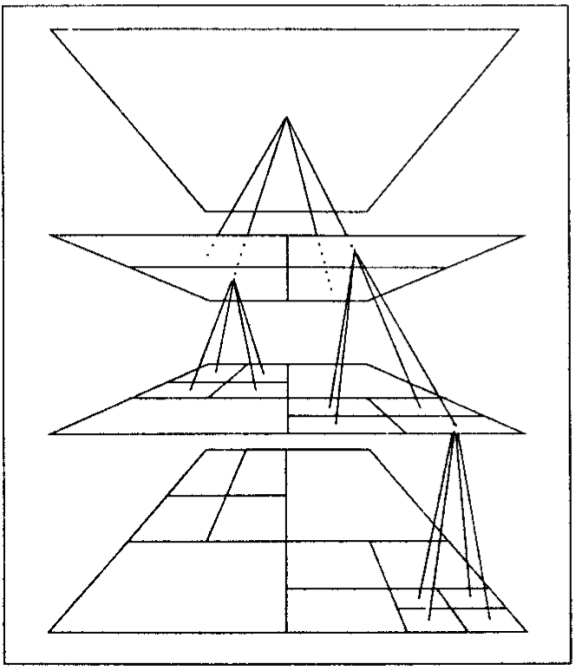
\includegraphics[width=0.3\textwidth]{pic3}
    \caption{Quadtree-based fractal encoding scheme}
    \label{fig:quadtree}
\end{figure}

\paragraph{Transformation}
In this section, we aim to create contraction mappings from \( D_k \) to \( R_l \). Our objective is to find a mapping \( f_l \) so that \( f(x_{D_k}) \) approximates \( x_{R_l} \) as closely as possible. In other words, we hope to find a mapping that makes \( D_k \) and \( R_l \) very similar after the transformation. Clearly, the more mappings we generate, the higher the likelihood of finding a suitable one. However, an excessively large set of functions \( f_l \) will reduce compression efficiency. Therefore, there is a trade-off: the more mappings we have, the better the potential matches, but at the cost of more storage space required for the mappings.

The mapping we choose here has the following form:
\[
f_l (x_{D_k}) = s \times \text{rotate}_\theta (\text{flip}_d (\text{reduce}(x_{D_k}))) + b
\]

And here is the pseudocode of how to apply transformation.
\begin{algorithm}
\caption{Implement Transformation}
\begin{algorithmic}[1]
\REQUIRE image, angle, direction, contrast = 1.0, brightness = 0.0
\STATE // Apply flipping, rotating, contrast adjustment, and brightness adjustment
\STATE transformed\_image = flip(image, direction)
\STATE // Flip the image horizontally or vertically based on direction
\STATE transformed\_image = rotate(transformed\_image, angle)
\STATE // Rotate the image by a given angle (90, 180, 270 degrees)
\STATE transformed\_image = contrast * transformed\_image + brightness
\RETURN transformed\_image
\end{algorithmic}
\end{algorithm}


\subsubsection{Compression}
After determining the method of transformation, we need to start compressing the image. According to the previous approach, we first generate all affine transformations of the domain blocks. And for each range block, we identify the best corresponding domain block and optimize its contrast and brightness.
Finally, we return the best transformation parameters for all range blocks to achieve image compression.

% Generate transformed blocks
\begin{algorithm}
\caption{Generate Transformed Block Set}
\begin{algorithmic}[1]
\REQUIRE image, source\_size, destination\_size, step
\STATE factor $\gets$ source\_size // destination\_size \textcolor{gray}{// Calculate scaling factor}
\STATE transformed\_blocks $\gets$ empty list \textcolor{gray}{// Initializes an empty list to store all the transformed blocks}
\FOR{each source block in image}
    \STATE S $\gets$ reduce(source block, factor) \textcolor{gray}{// Reduce source block}
    \FOR{each transformation in candidates}
        \STATE transformed $\gets$ apply\_transform(S, transformation) % Apply transformation
        \STATE add (position, transformation, transformed) to transformed\_blocks \textcolor{gray}{//Add transformation info into transformed blocks}
    \ENDFOR
\ENDFOR
\RETURN transformed\_blocks
\end{algorithmic}
\end{algorithm}

% Explanation of the compression process
Following is the \texttt{compress} function. It iterates over each destination block in the image, extracts it, and tests all the previously generated transformed source blocks to find the best match. The best match is determined by optimizing the contrast and brightness using the \texttt{find\_contrast\_and\_brightness2} function, which solves a least squares problem to fit the contrast and brightness. The function returns the best transformation parameters for all destination blocks, achieving image compression.

\begin{algorithm}
\caption{Compress Image}
\begin{algorithmic}[1]
\REQUIRE img, source\_size, destination\_size, step
\STATE transformations $\gets$ empty list
\STATE transformed\_blocks $\gets$ generate\_all\_transformed\_blocks(img, source\_size, destination\_size, step)
\FOR{each destination block position (i, j) in img}
    \STATE add empty list to transformations[i]
    \STATE min\_d $\gets$ infinity
    \STATE D $\gets$ extract\_destination\_block(img, i, j, destination\_size) \textcolor{gray}{//D is the destination block}
    \FOR{each transformed block in transformed\_blocks}
        \STATE S $\gets$ transformed block \textcolor{gray}{//Now S is the new transformed block}
        \STATE (contrast, brightness) $\gets$ find\_contrast\_and\_brightness2(D, S) \textcolor{gray}{//Find the best contrast and brightness for S and D}
        \STATE S $\gets$ contrast $\times$ S + brightness \textcolor{gray}{//Adjust S}
        \STATE d $\gets$ compute\_difference(D, S) \textcolor{gray}{//Compute difference}
        \IF{d \textless  min\_d}
            \STATE min\_d $\gets$ d
            \STATE transformations[i][j] $\gets$ (k, l, direction, angle, contrast, brightness) \textcolor{gray}{//Save the best transformation parameters for current D}
        \ENDIF
    \ENDFOR
\ENDFOR
\RETURN transformations
\end{algorithmic}
\end{algorithm}
\begin{algorithm}
\caption{Image Compression Algorithm}
\begin{algorithmic}[1]
\REQUIRE image, source\_size, destination\_size, stride
\STATE transform\_list $\gets$ empty list
\STATE transformed\_blocks $\gets$ generate\_transformed\_blocks(image, source\_size, destination\_size, stride)
\FOR{each target block position (x, y) in image}
    \STATE add empty list to transform\_list[x]
    \STATE min\_difference $\gets$ infinity
    \STATE target\_block $\gets$ extract\_target\_block(image, x, y, destination\_size) \textcolor{gray}{// target\_block represents the destination block}
    \FOR{each transformed\_block in transformed\_blocks}
        \STATE source\_block $\gets$ transformed\_block \textcolor{gray}{// source\_block is the current transformed block}
        \STATE (contrast, brightness) $\gets$ compute\_contrast\_brightness(target\_block, source\_block) \textcolor{gray}{//Compute optimal contrast and brightness for the blocks}
        \STATE source\_block $\gets$ contrast $\times$ source\_block + brightness \textcolor{gray}{//Adjust the source block}
        \STATE difference $\gets$ calculate\_difference(target\_block, source\_block) \textcolor{gray}{//Calculate the difference}
        \IF{difference \textless  min\_difference}
            \STATE min\_difference $\gets$ difference
            \STATE transform\_list[x][y] $\gets$ (index, rotation, flip, scale, contrast, brightness) \textcolor{gray}{//Store the optimal transformation parameters for the current block}
        \ENDIF
    \ENDFOR
\ENDFOR
\RETURN transform\_list
\end{algorithmic}
\end{algorithm}

\FloatBarrier
\subsubsection{Decompression}

Algorithm 9 outlines the process of decompressing an image using a series of transformations. The algorithm starts by calculating the scaling factor between the source and destination sizes. It then determines the dimensions of the resulting image and initializes with a random image. A series of iterations are performed to apply the transformations.

In each iteration, the algorithm iterates through the transformation grid. For each cell in the grid, it retrieves the transformation parameters, reduces the source block, applies the transformation, and updates the current image with the transformed block. After completing all transformations for an iteration, the current image is saved, and the image is reset for the next iteration. This process repeats for a specified number of iterations. Finally, the algorithm returns all iterations of the decompressed images.
\begin{algorithm}
\caption{Decompress Image}
\begin{algorithmic}[1]
\REQUIRE transformations, source\_size, destination\_size, stride, num\_iterations=8
\STATE scale\_factor $\gets$ \texttt{source\_size // destination\_size} \textcolor{gray}{// Calculate scaling factor}
\STATE img\_height $\gets$ \texttt{len(transformations) $\times$ destination\_size} \textcolor{gray}{// Determine image height}
\STATE img\_width $\gets$ \texttt{len(transformations[0]) $\times$ destination\_size} \textcolor{gray}{// Determine image width}
\STATE iterations $\gets$ [\texttt{np.random.randint(0, 256, (img\_height, img\_width))}] \textcolor{gray}{// Initialize with a random image}
\STATE current\_image $\gets$ \texttt{np.zeros((img\_height, img\_width))} \textcolor{gray}{// Initialize current image}
\FOR{iter $\gets$ 0 \textbf{to} num\_iterations}
    \FOR{x $\gets$ 0 \textbf{to} \texttt{len(transformations)}}
        \FOR{y $\gets$ 0 \textbf{to} \texttt{len(transformations[x])}}
            \STATE (src\_x, src\_y, flip, rotate, contrast, brightness) $\gets$ transformations[x][y] \textcolor{gray}{// Retrieve transformation parameters}
            \STATE Reduce the source block \textcolor{gray}{// Downscale the source block}
            \STATE Apply the transformation \textcolor{gray}{// Transform the block}
            \STATE Update the current image \textcolor{gray}{// Insert into current image}
        \ENDFOR
    \ENDFOR
    \STATE Save the current image \textcolor{gray}{// Record iteration result}
    \STATE Reset the current image \textcolor{gray}{// Clear for next iteration}
\ENDFOR
\RETURN iterations \textcolor{gray}{// Return all iterations}
\end{algorithmic}
\end{algorithm}


\subsubsection{Issues and Idea of Improvement}

The theoretical basis of fractal compression methods is Iterated Function Systems (IFS) theory. However, this methods also has several disadvantages:

1. \textbf{Long Encoding Time}: The extensive search and matching required for encoding lead to long processing times.

2. \textbf{Lower Compression Ratio}: The compression ratio is not as high because the method does not comprehensively consider global and local similarities. This limitation results in significant constraints in simple block-to-block transformations.

To address these disadvantages, improvements can be focused on the following areas:

1. \textbf{Enhancing Compression Ratio and Compression Effect}: By developing more sophisticated algorithms that better capture the similarities within and across frames, the compression ratio and overall effect can be improved.

2. \textbf{Increasing Encoding Speed}: Optimization techniques such as parallel processing, more efficient search algorithms, and hardware acceleration can significantly reduce encoding times.

3. \textbf{Increasing Decoding Speed}: Some optimization techniques can also be applied to the decoding process to enhance its speed.

\paragraph{Enhancing Compression Ratio and Compression Effect}

According to theoretical analysis, the size of the domain blocks and range blocks has a significant impact on the quality and compression ratio of fractal image coding. Considering two extreme cases: if the domain block is \(2^D \times 2^D\) pixels and the range block is \(2^R \times 2^R\) pixels, when \(D\) and \(R\) are very large, although the number of domain blocks in the domain block library is relatively large, it is difficult to find a high similarity between the range block and the domain block, resulting in poor image quality after decoding. Conversely, if \(D\) and \(R\) are very small, the smallest case being a range block of one pixel and a domain block of four pixels, it is always possible to find a very good similarity match coefficient, but the number of affine transformations required for image coding increases sharply, failing to achieve the purpose of compression.\\
Therefore, Fisher and Jacquin proposed an adaptive adjustment method, which improves the coding effect and compression ratio by changing the size of the range blocks and domain blocks. The key to this method is to use a tolerable error (\( \varepsilon \)) to decide the size adjustment of the blocks.
Here is the idea and pseudocode of the method of improvement

\textbf{Adaptive Quadtree Coding Method}\cite{128028}\cite{Fisher1995}

1. \textbf{Adjusting Block Size}
   \begin{itemize}
       \item For large domain blocks and range blocks, choose appropriate affine transformation coefficients.
       \item For large blocks where a good match cannot be found, progressively reduce the block size from \( 2^R \) to \( 2^{R-1} \), \( 2^{R-2} \), and so on.
   \end{itemize}

We should have a new transformation that we may use:


\begin{algorithm}
\caption{Enlarge Image by a Factor}
\begin{algorithmic}[1]
\STATE Initialize a zero matrix \texttt{result} with dimensions $(\text{img.shape}[0] \times \text{factor}, \text{img.shape}[1] \times \text{factor})$
\FOR{each $i$ in range(\texttt{result.shape}[0])}
    \FOR{each $j$ in range(\texttt{result.shape}[1])}
        \STATE Set \texttt{result[i, j]} to \texttt{img[i // factor, j // factor]}
    \ENDFOR
\ENDFOR
\RETURN \texttt{result}
\end{algorithmic}
\end{algorithm}

Then we use quadtree\_decompose function to decompose the image to several partitions.

\begin{algorithm}
\caption{Quadtree Decomposition}
\begin{algorithmic}[1]
\STATE Define the quadtree decomposition function:
\STATE $\texttt{quadtree\_decompose(img, threshold=256, min\_size=2)}$
\STATE Initialize \texttt{decompose} function: \quad \texttt{decompose(block, x, y, size, threshold)}
\IF{size $\leq$ min\_size \textbf{or} \texttt{variance(block)} $\leq$ threshold}
    \RETURN $[(x, y, size)]$
\ENDIF

\STATE Calculate half size: \quad \texttt{half = size // 2}
\RETURN Concatenate decomposed blocks:
\STATE \quad \texttt{decompose(block[:half, :half], x, y, half, threshold)} $+$
\STATE \quad \texttt{decompose(block[:half, half:], x, y + half, half, threshold)} $+$
\STATE \quad \texttt{decompose(block[half:, :half], x + half, y, half, threshold)} $+$
\STATE \quad \texttt{decompose(block[half:, half:], x + half, y + half, half, threshold)}

\STATE Return the result of \texttt{decompose(img, 0, 0, img.shape[0], threshold)}

\end{algorithmic}
\end{algorithm}


\begin{figure}[ht]
    \centering
    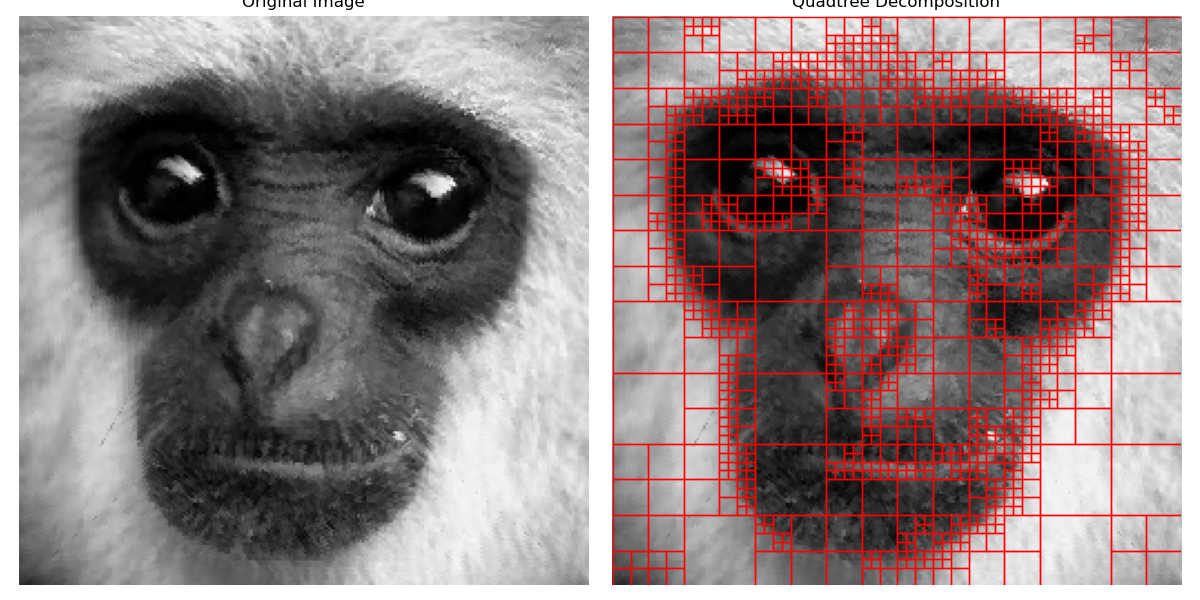
\includegraphics[width=\textwidth]{quadtree_comparison.png}
    \caption{Comparison of Original Image and Quadtree Decomposition}
    \label{fig:quadtree_comparison}
\end{figure}

This process ensures that each block in the quadtree is either uniform enough (low variance) or small enough (minimum size), resulting in an efficient and adaptive partitioning of the image. Figure \ref{fig:quadtree_comparison} is an example of the partition.

2. \textbf{Compression}

The idea is same with the traditional compression
  
\textbf{1. Generate All Transformed Blocks:}
\begin{itemize}
    \item Use the \texttt{generate\_all\_transformed\_blocks\_quadtree} function to generate all possible transformed blocks.
    \item Transformations include rotations (0°, 90°, 180°, 270°) and flips (horizontal flip, vertical flip).
    \item Apply the above transformations to each quadtree block to generate the transformed blocks.
\end{itemize}

\begin{algorithm}
\caption{Generate All Transformed Blocks Quadtree}
\begin{algorithmic}[1]
\STATE Initialize an empty list \texttt{transformed\_blocks}
\FOR{each $(x, y, \text{size\_s})$ in \texttt{quadtree\_blocks}}
    \STATE Extract block $S$ from $img$ at coordinates $(x:x+\text{size\_s}, y:y+\text{size\_s})$
    \FOR{each \texttt{direction} in $[1, -1]$}
        \FOR{each \texttt{angle} in $[0, 90, 180, 270]$}
            \STATE Apply transformation to $S$ using \texttt{direction} and \texttt{angle} to get \texttt{transformed\_S}
            \STATE Append $(x, y, \text{size\_s}, \text{direction}, \text{angle}, \text{transformed\_S})$ to \texttt{transformed\_blocks}
        \ENDFOR
    \ENDFOR
\ENDFOR
\RETURN \texttt{transformed\_blocks}
\end{algorithmic}
\end{algorithm}

\newpage


\textbf{2. Compression Processing:}
\begin{algorithm}
\caption{Compress with Quadtree - Part 1: Initialization}
\begin{algorithmic}[1]
\STATE Initialize quadtree blocks with \texttt{quadtree\_decompose(img, threshold, min\_size)}
\STATE Initialize \texttt{transformations} as an empty list
\STATE Generate all transformed blocks with \texttt{generate\_all\_transformed\_blocks\_quadtree}
\end{algorithmic}
\end{algorithm}
\begin{itemize}
    \item Iterate through each quadtree block and find the best matching transformed block.

\begin{algorithm}
\caption{Compress with Quadtree - Part 2: Process Each Block}
\begin{algorithmic}[1]
\FOR{each block $(x, y, size)$ in \texttt{quadtree\_blocks}}
    \STATE Extract block $D$ from \texttt{img[x:x+size, y:y+size]}
    \STATE Initialize \texttt{min\_d} to $\infty$
    \STATE Initialize \texttt{best\_transform} to \texttt{None}
\ENDFOR
\end{algorithmic}
\end{algorithm}

    \item To find the best matching block, resize each candidate transformed block to match the current block size.


    \item Calculate the contrast and brightness adjustment coefficients to make the transformed block as close as possible to the current block.
    \item Compute the difference between the adjusted block and the current block, and choose the block with the smallest difference as the best matching block.
\end{itemize}
\begin{algorithm}
\caption{Compress with Quadtree - Part 3: Find Best Transformation}
\begin{algorithmic}[1]
    \FOR{each transformed block $(k, l, size\_s, direction, angle, S)$ in \texttt{transformed\_blocks}}
        \IF{$size\_s \leq size$}
            \STATE \texttt{continue}
        \ELSE
            \STATE Enlarge $D$ to match $size\_s$
        \ENDIF
        \STATE Calculate contrast and brightness with \texttt{find\_contrast\_and\_brightness2(D\_t, S)}
        \STATE Transform $S$ with calculated contrast and brightness
        \STATE Calculate difference $d$ between $D\_t$ and transformed $S$
        \IF{$d < \texttt{min\_d}$}
            \STATE Update \texttt{min\_d} and \texttt{best\_transform}
        \ENDIF
    \ENDFOR
\end{algorithmic}
\end{algorithm}


\textbf{3. Record the Best Transformations:}
\begin{itemize}
    \item handle largest blocks in decomposition.
    \item For each quadtree block, record its best transformation parameters, including position, size, rotation angle, flip direction, contrast, and brightness adjustment coefficients.
\end{itemize}


\begin{algorithm}
\caption{Compress with Quadtree - Part 4: Handle No Best Transformation and record best transformations}
\begin{algorithmic}[1]
    \IF{\texttt{best\_transform} is \texttt{None}}
        \STATE compare with larger size block divided by traditional method, and find best matching. 
    \ENDIF
    \STATE Append \texttt{best\_transform} to \texttt{transformations}
\end{algorithmic}
\end{algorithm}

3. \textbf{Decompression}

Decompression is simple, we just put these transformed blocks
to the destination position and destination size. 

\begin{algorithm}
\caption{Decompress with Quadtree}
\begin{algorithmic}[1]
\STATE Initialize \texttt{height}, \texttt{width}, \texttt{transformations} from \texttt{compressed\_code}

\STATE Initialize \texttt{iterations} with a random matrix of size \texttt{height} $\times$ \texttt{width}
\STATE Initialize \texttt{cur\_img} as a zero matrix of size \texttt{height} $\times$ \texttt{width}

\FOR{\texttt{i\_iter} in \texttt{range(number of iter)}}
    \FOR{all data stored \textbf{in} \texttt{transformations}}
        \STATE Set \texttt{S} to \texttt{iterations[-1][k:k+size\_s, l:l+size\_s]}
        \STATE Set \texttt{D} to \texttt{apply\_transformation(S, direction, angle, contrast, brightness)}
        \IF{\texttt{size\_s} $\neq$ \texttt{size}}
            \STATE adjust size of D to fit size of destination
        \ENDIF
        \STATE Set \texttt{cur\_img[x:x+size, y:y+size]} to \texttt{D}
    \ENDFOR
    \STATE Append \texttt{cur\_img} to \texttt{iterations}
\ENDFOR
\RETURN \texttt{iterations}
\end{algorithmic}
\end{algorithm}

It is easy to get that Quadtree optimization offers significant benefits in image compression:

\begin{itemize}
    \item \textbf{Adaptive Resolution Handling}: Quadtree decomposition allows variable block sizes, representing uniform areas with larger blocks and complex areas with smaller blocks, providing fine-grained control over image resolution.
    \item \textbf{Improved Compression Efficiency}: By merging similar areas into larger blocks, quadtree reduces redundancy and achieves higher compression ratios without significant quality loss.
    \item \textbf{Optimized Computational Load}: Selective processing of image regions based on variance and size criteria reduces computational load compared to uniform processing methods.
\end{itemize}

Overall, quadtree optimization improves compression ratios, reduces computational load, and preserves image quality effectively.

\paragraph{Increasing the Encoding Speed}

To reduce the complexity of searching during fractal coding, there are two main methods:

1. Reducing the search range of the domain blocks: This method changes the global search matching to neighborhood search matching. When constructing the fractal code for the range block, it only searches within the neighborhood of the corresponding domain block. This method is suitable for images that meet the near-distance self-similarity model.

2. Classifying domain blocks and range blocks: This method classifies domain blocks and range blocks, changing the global search matching to class-based search matching. Therefore, when constructing the fractal transform corresponding to the range block, it only searches within the same class of domain blocks.

Both of the above methods replace the global optimal matching with local optimal matching. In practical applications, the more classifications there are, the shorter the encoding time for class matching fractal blocks, but the lower the quality of the decoded image. Similarly, the smaller the neighborhood range, the larger the search step size, the shorter the encoding time for neighborhood matching fractal blocks, but the lower the relative quality of the decoded image.

\textbf{Method 1: Reducing the Search Range of Domain Blocks}
This method modifies the global search matching to neighborhood search matching. When constructing the fractal code corresponding to a range block, it only searches within the neighborhood of the corresponding domain block. This approach is suitable for images that meet the near-distance self-similarity model.

To implement the neighborhood search optimization in the compression algorithm, we need to modify the code to restrict the search range of domain blocks to a local neighborhood around the range block currently being processed.

\begin{itemize}
    \item Define the Neighborhood: Specify a neighborhood size to define the local search area around the current range block. This could be a fixed size or a proportion of the image size.
    \item Modify the Search Loop: 1. Instead of searching all domain blocks in the image, restrict the search to domain blocks within the defined neighborhood around the range block. 2. Adjust the \texttt{generate\_all\_transformed\_blocks} function to consider only the domain blocks within this neighborhood.

\begin{algorithm}
\caption{Generate All Transformed Blocks with Neighborhood Search}
\begin{algorithmic}[1]
\STATE Initialize an empty list \texttt{transformed\_blocks}
\FOR{each destination block starting at $(i, j)$ in the image with step \texttt{destination\_size}}
    \STATE Add an empty list to \texttt{transformed\_blocks}
    \FOR{each source block starting at $(k, l)$ within the neighborhood around $(i, j)$}
        \STATE Extract the source block $S$ and reduce it to the shape of a destination block
        \STATE apply each transformation to the block
        \STATE append each transformed block in to \texttt{(i, j)} of   \texttt{transformed\_blocks}
    \ENDFOR
\ENDFOR
\RETURN \texttt{transformed\_blocks}
\end{algorithmic}
\end{algorithm}

    \item Modify the \texttt{compress} function to incorporate the neighborhood search logic. This involves calling the updated \texttt{generate\_all\_transformed\_blocks function} and processing the restricted domain blocks for each range block.
    \item The decompression process is same with the original method.
\end{itemize}

 Obviously, by limiting the search to neighboring blocks, the method significantly reduces the computational complexity and time required for encoding. And this method is more efficient for images with strong local self-similarity, as it avoids the need to search the entire image.

However, The quality of the reconstructed image may be lower compared to global search methods, as the optimal match might be outside the local neighborhood. And also, the effectiveness of this method is highly dependent on the image characteristics. It may not perform well for images lacking local self-similarity. The next method may suitable for all type of image.

\textbf{Method 2: Classify Domain Blocks and Range Blocks}
In order to improve encoding speed, this method involves classifying both domain blocks and range blocks. By classifying, we transform the global search into a more efficient search within the same class. This means that during the construction of the fractal transformation corresponding to a range block, the search for the optimal matching block is confined to the same class of domain blocks. This approach reduces the overall search space, making the encoding process faster.

A classical way to classify the domain and range of the image is variance (which we used in previous part to take quadtree partitions).
Since regions with high variance have more detail (complicated area), but regions with low variance have ess detail (smooth area).
We can classify blocks of image to several groups by variance, and only compare blocks in the same group (figure \ref{fig:classification} is an example of block classification of image, where  \text{Group 0} = \{ \text{blocks} \mid \text{variance} < 128 \}, \text{Group 1} = \{ \text{blocks} \mid 128 < \text{variance} < 256 \},  \text{Group 2} = \{ \text{blocks} \mid 256 < \text{variance} < 512 \},  \text{Group 3} = \{ \text{blocks} \mid 512 < \text{variance} < 1024 \},  \text{Group 14} = \{ \text{blocks} \mid \text{variance} > 1024\}.) 

\begin{figure}[H]
    \centering
    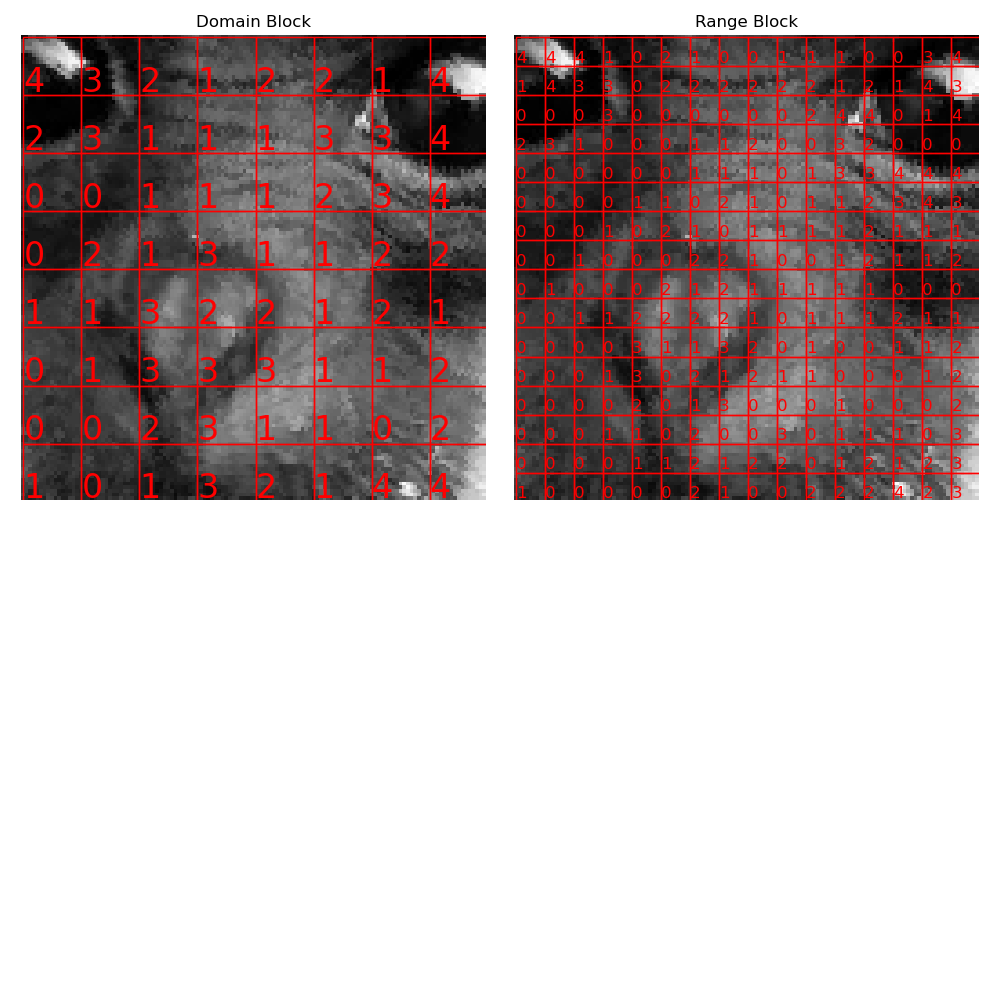
\includegraphics[width=\textwidth, trim=0 350 0 0,clip]{classification.png}
    \caption{blocks of an image classified by variance}
    \label{fig:classification}
\end{figure}

To optimize the fractal compression algorithm by classifying blocks based on their variance, we will modify the code to include the following steps:

\begin{itemize}
    \item Implement a Function to Classify Blocks by Variance: Blocks will be categorized into different classes according to predefined variance thresholds.

\begin{algorithm}
\caption{Classify Variance}
\begin{algorithmic}[1]
    \REQUIRE  $block$, $thresholds$
    \ENSURE $class\_label$
    \FOR{$i, threshold$ \textbf{in} \text{enumerate}($thresholds$)}
        \IF{$var of block < threshold$}
            \RETURN $i$
        \ENDIF
    \ENDFOR
    \RETURN \text{len}($thresholds$)
\end{algorithmic}
\end{algorithm}
    \item Modify the \texttt{generate\_all\_transformed\_blocks} Function: generating all transformed blocks and classify them in several groups. 

\begin{algorithm}
\caption{Generate All Transformed Blocks with Classification}
\begin{algorithmic}[1]
\REQUIRE img, source\_size, destination\_size, step, thresholds
\ENSURE Transformed Blocks for each class
\STATE Initialize an empty list \texttt{transformed\_blocks}
\STATE Generating len(thresholds) empty lists in \texttt{transformed\_blocks}
\STATE Compute \texttt{factor} as \texttt{source\_size // destination\_size}
\FOR{every source blocks}
    \STATE Extract the source block \texttt{S} and reduce it to the shape of a destination block
    \STATE Classify \texttt{S} based on its variance
    \STATE $class\_label \leftarrow \texttt{classify\_variance(S, thresholds)}$
    \FOR{$(direction, angle)$ in \{(1, 0), (1, 90), (1, 180), (1, 270), (-1, 0), (-1, 90), (-1, 180), (-1, 270)\}}
        \STATE Generate transformed block and append to the corresponding class list
    \ENDFOR
\ENDFOR
\RETURN \texttt{transformed\_blocks}
\end{algorithmic}
\end{algorithm}

    \item Modify the Compression Function: Ensure that the compression algorithm searches for matching blocks within the same variance class only, reducing the search space and improving efficiency.

    \item Decompression does not change, because transformations generated in compression function is same as the original method.
\end{itemize}

\begin{algorithm}
\caption{Compress with Classification}
\begin{algorithmic}[1]
\STATE Initialize empty list $transformations$
\STATE Generate all transformed blocks using the function generate\_all\_transformed\_blocks\_class
\FOR{all destination blocks}
    \STATE Classify the destination block by variance.
    \STATE $class\_label \gets classify\_variance(D, thresholds)$
    \FOR{each $(k, l, direction, angle, S)$ in $transformed\_blocks[class\_label]$}
        \STATE Find the best matching block
        \STATE $transformations[i][j] \gets (k, l, direction, angle, contrast, brightness)$
    \ENDFOR
\ENDFOR
\RETURN $transformations$
\end{algorithmic}
\end{algorithm}


By figure \ref{fig:classification_based_compress}, it is easy to see that the classification based compression is faster than the original compression (global compression). 
This is because by limiting the search for matching blocks to those within the same variance class, the method significantly reduces the number of comparisons required. And the method is more efficient for images with strong local self-similarity, as it avoids unnecessary comparisons with dissimilar blocks.

\begin{figure}[H]
    \centering
    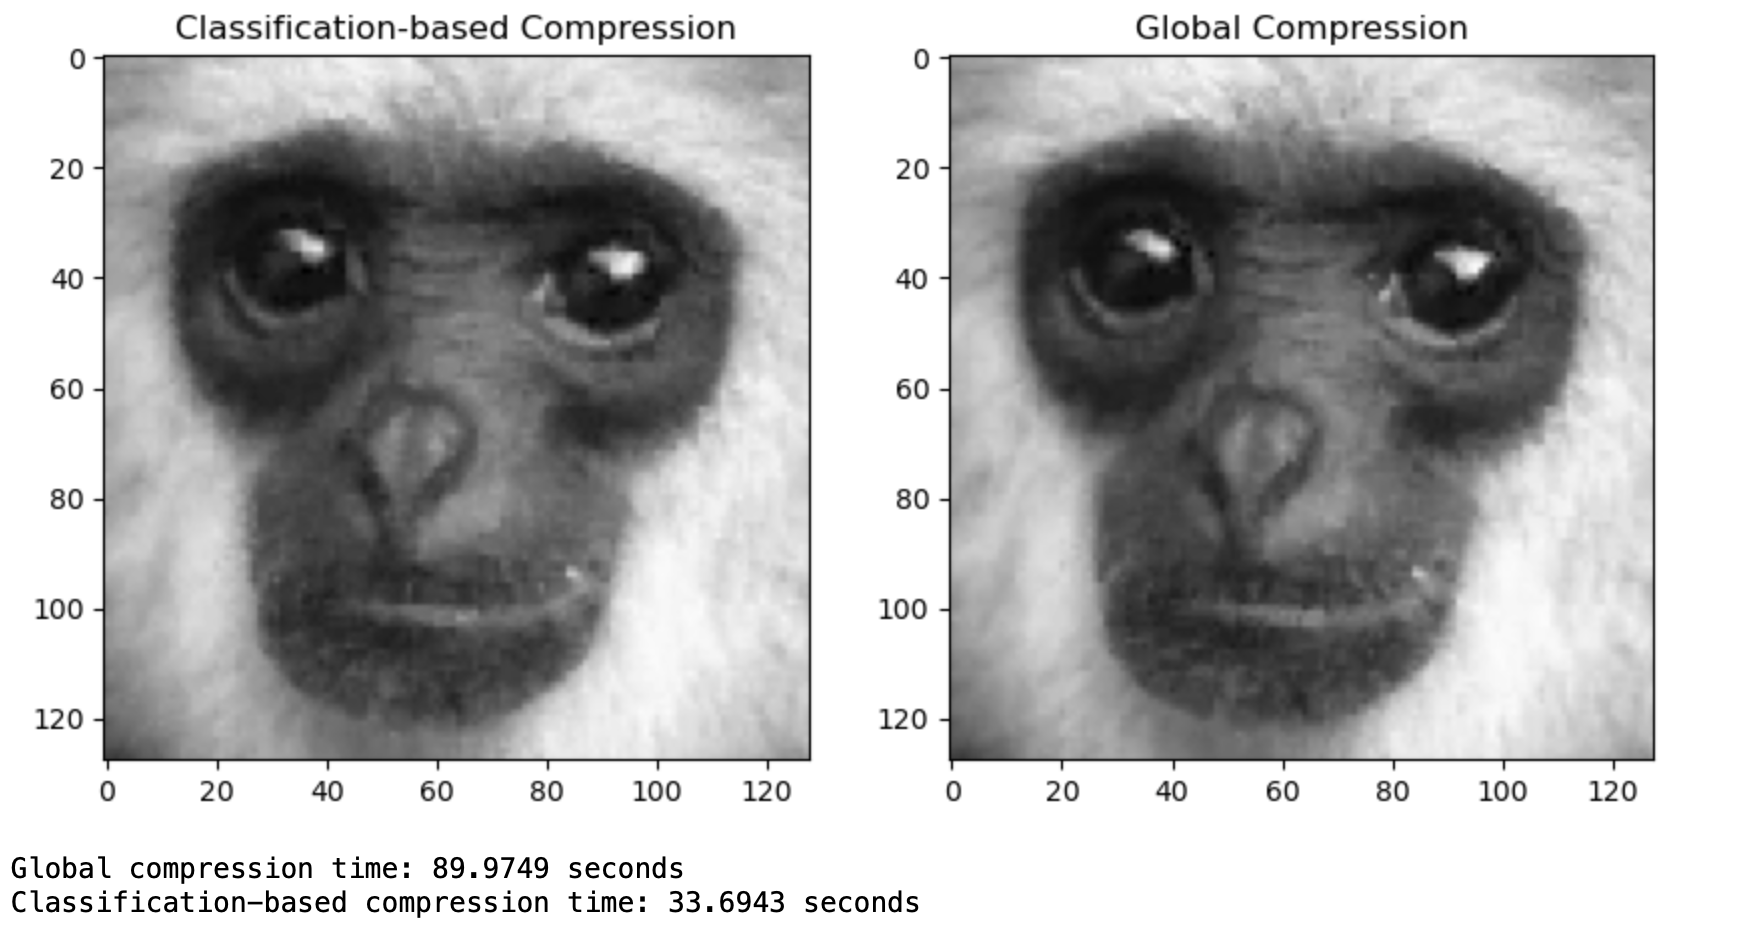
\includegraphics[width=\textwidth]{classification_based_compress.png}
    \caption{classification based compression}
    \label{fig:classification_based_compress}
\end{figure}

\paragraph{Increasing the Decoding Speed}

From the automatic fractal image encoding algorithm, it can be seen that during decoding, selecting about ten iterations is generally sufficient to reconstruct the original image. However, in practical applications, fewer iterations are preferred for better performance, which can further reduce decoding time and improve decoding speed. There is an easy way to deal with it.

\textbf{Mean Subtraction Decoding Method}

The mean subtraction decoding method is an optimization technique used in fractal image compression to enhance decoding efficiency. It involves the following steps:
\begin{itemize}
    \item Calculate the mean value of the pixels in each block, and subtract the mean value from each block to obtain the mean subtracted block.
    \item Compression process is totally same with the general method.
    \item Decompression process: 1. Reconstruct the image block by block based on the recorded transformation parameters. 2. After each iteration, add back the mean value of the mean-subtracted block to restore the original brightness level.
\end{itemize}

\begin{figure}
    \centering
    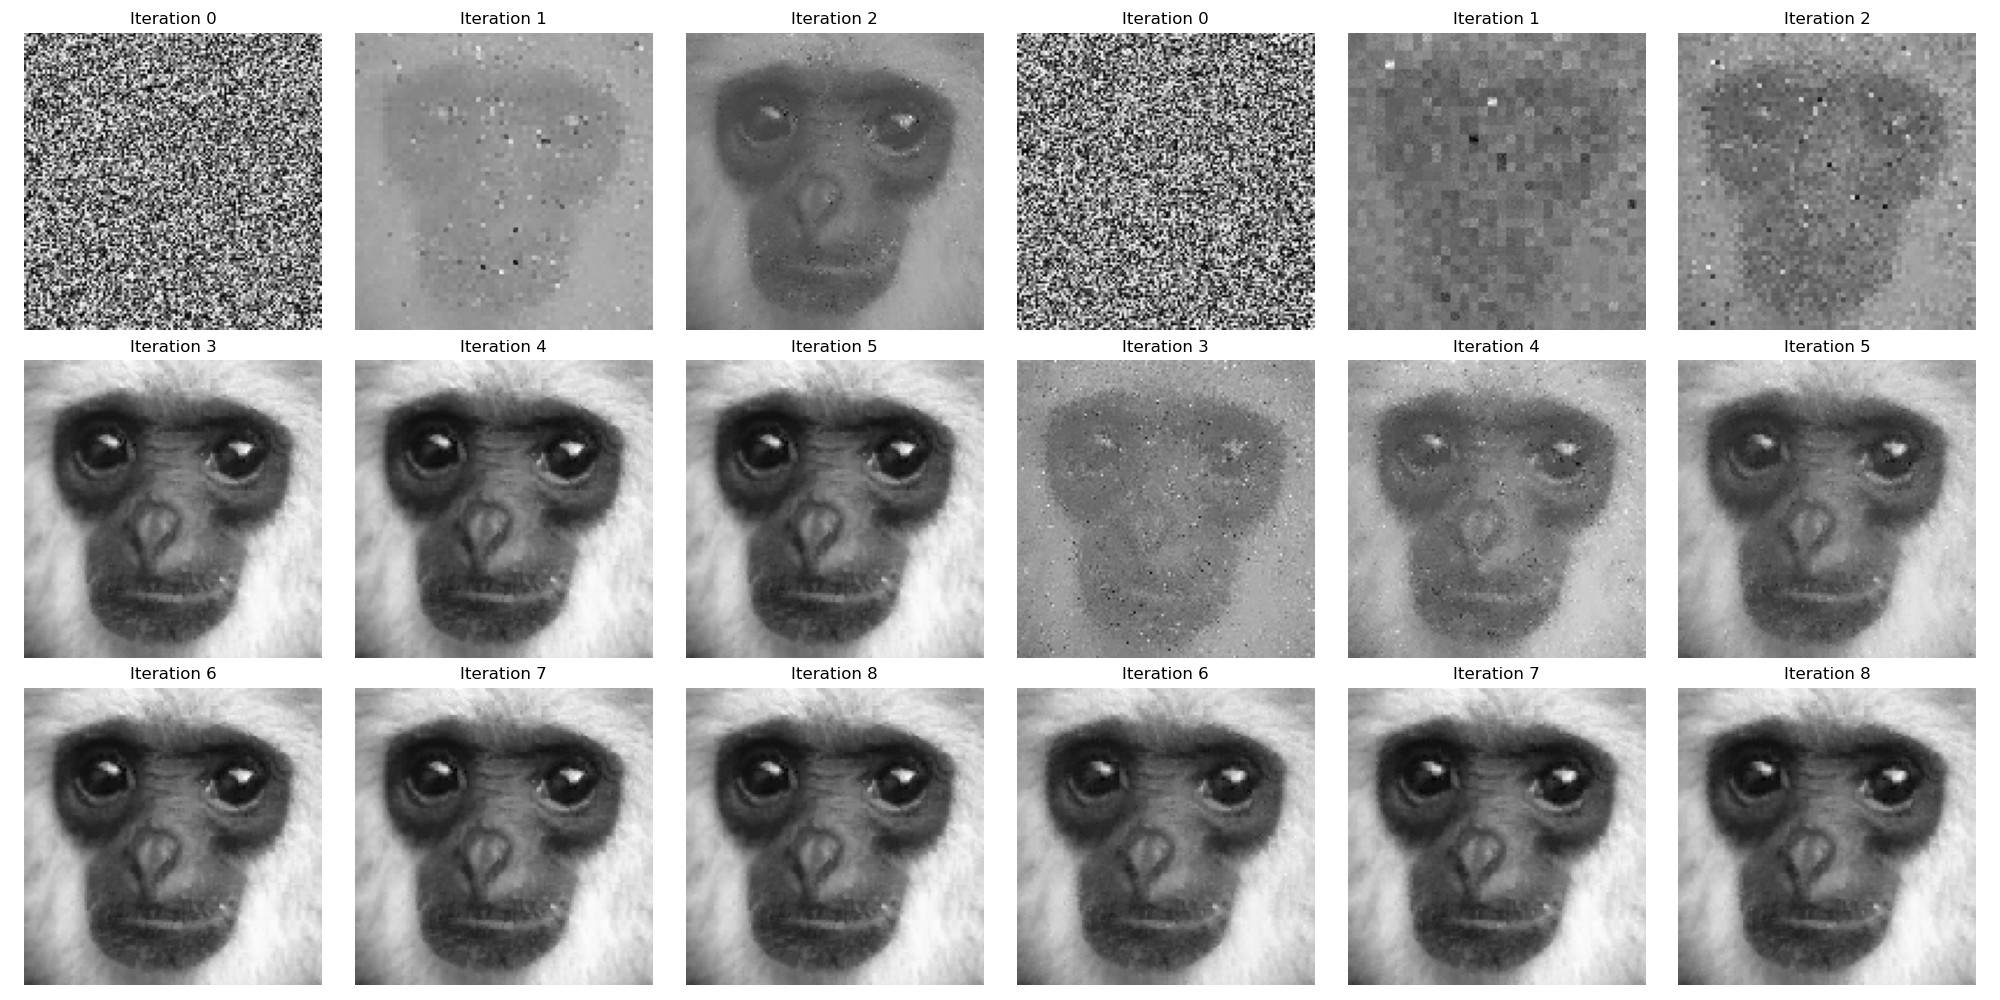
\includegraphics[width=\textwidth]{Mean Subtraction.png}
    \caption{First set is iterations decompressed by mean subtraction method, second set is iterations decompressed by general method}
    \label{fig:Mean Subtraction}
\end{figure}

From the figure \ref{fig:Mean Subtraction}, we can clearly see that iterations decompressed by mean subtraction is converge faster than general method. This is because by subtracting the mean from each block, the dynamic range of the pixel values is reduced, making it easier to find a suitable match during the compression and decompression processes. 

\newpage
\subsection{Inverse IFS Problem}
The two algorithms discussed in section 3 are ways of computing the attractor when given an IFS. So the question that remains is when given an image can you determine an IFS for it, the motivation for this question is the fact that storing a set of affine transformations instead of the all pixels of the original image would be more efficient.We approached this question with two different ideas, which we will discuss in this section, focusing on finding writing a programme that will determine the IFS of the Sierpinski Triangle.

\subsubsection{K-means clustering}
Due to fractals being self-similar on all scales, our initial idea was to find a way to split the fractal apart into smaller similar versions, and from there compare these sets with the overall image. Focusing on the Sierpinski Triangle meant we knew what affine transformations we were hoping to find. 

Transformation 1 $=\begin{bmatrix} 0.5 &0\\0&0.5\end{bmatrix}\begin{bmatrix} x\\y \end{bmatrix} + \begin{bmatrix}0\\0\end{bmatrix}$
\\
Transformation 2 $=\begin{bmatrix} 0.5 &0\\0&0.5\end{bmatrix}\begin{bmatrix} x\\y \end{bmatrix} + \begin{bmatrix}0.5\\0\end{bmatrix}$
\\
Transformation 3 $=\begin{bmatrix} 0.5 &0\\0&0.5\end{bmatrix}\begin{bmatrix} x\\y \end{bmatrix} + \begin{bmatrix}\frac{\sqrt{3}}{2}\\0.5\end{bmatrix}$
\\

To split the fractal into self-similar shapes we used the method of clustering points. Cluster analysis is a technique used in machine learning to group similar objects into clusters. We decided to use K-means clustering, which partitions a dataset into a pre-defined number of clusters by minimizing the distance between data points and their assigned cluster’s center, called the centroid.\cite{sharma2019kmeans} This type of clustering clearly separates the fractal into the three self-similar shapes that have undergone the three affine transformations we are trying to find for the iterated function system.  

\begin{minipage}{0.45\textwidth}
       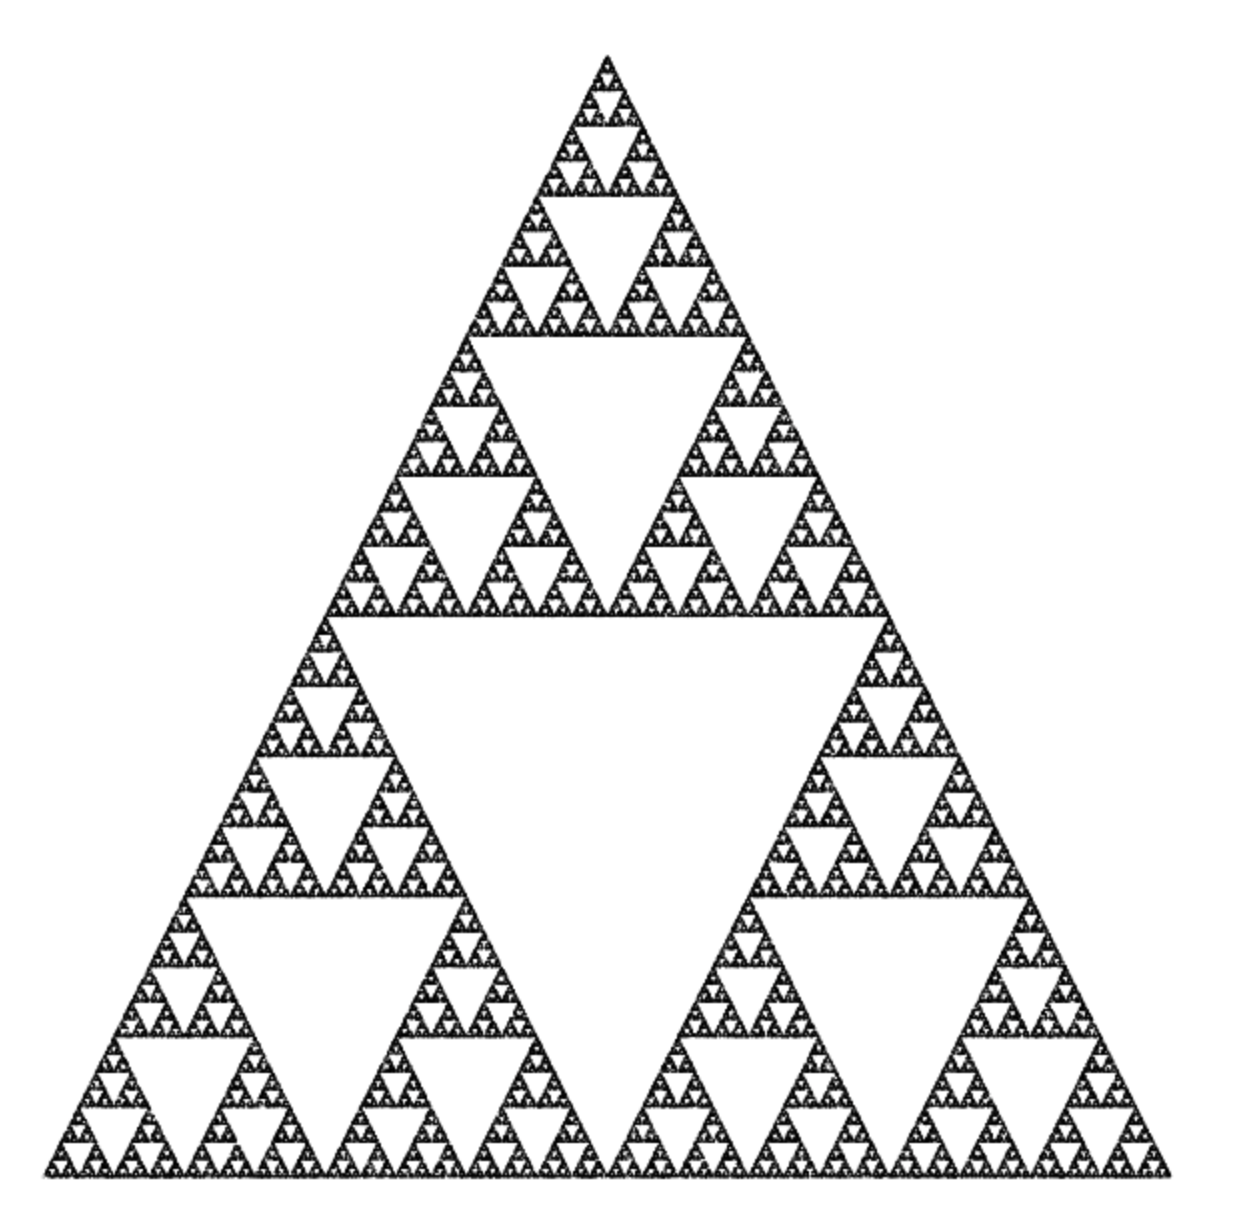
\includegraphics[width=8cm, height=8cm]{pic9.png}
       \captionof{figure}{Generated Image}
   \end{minipage}
   \hfill
   \begin{minipage}{0.45\textwidth}
       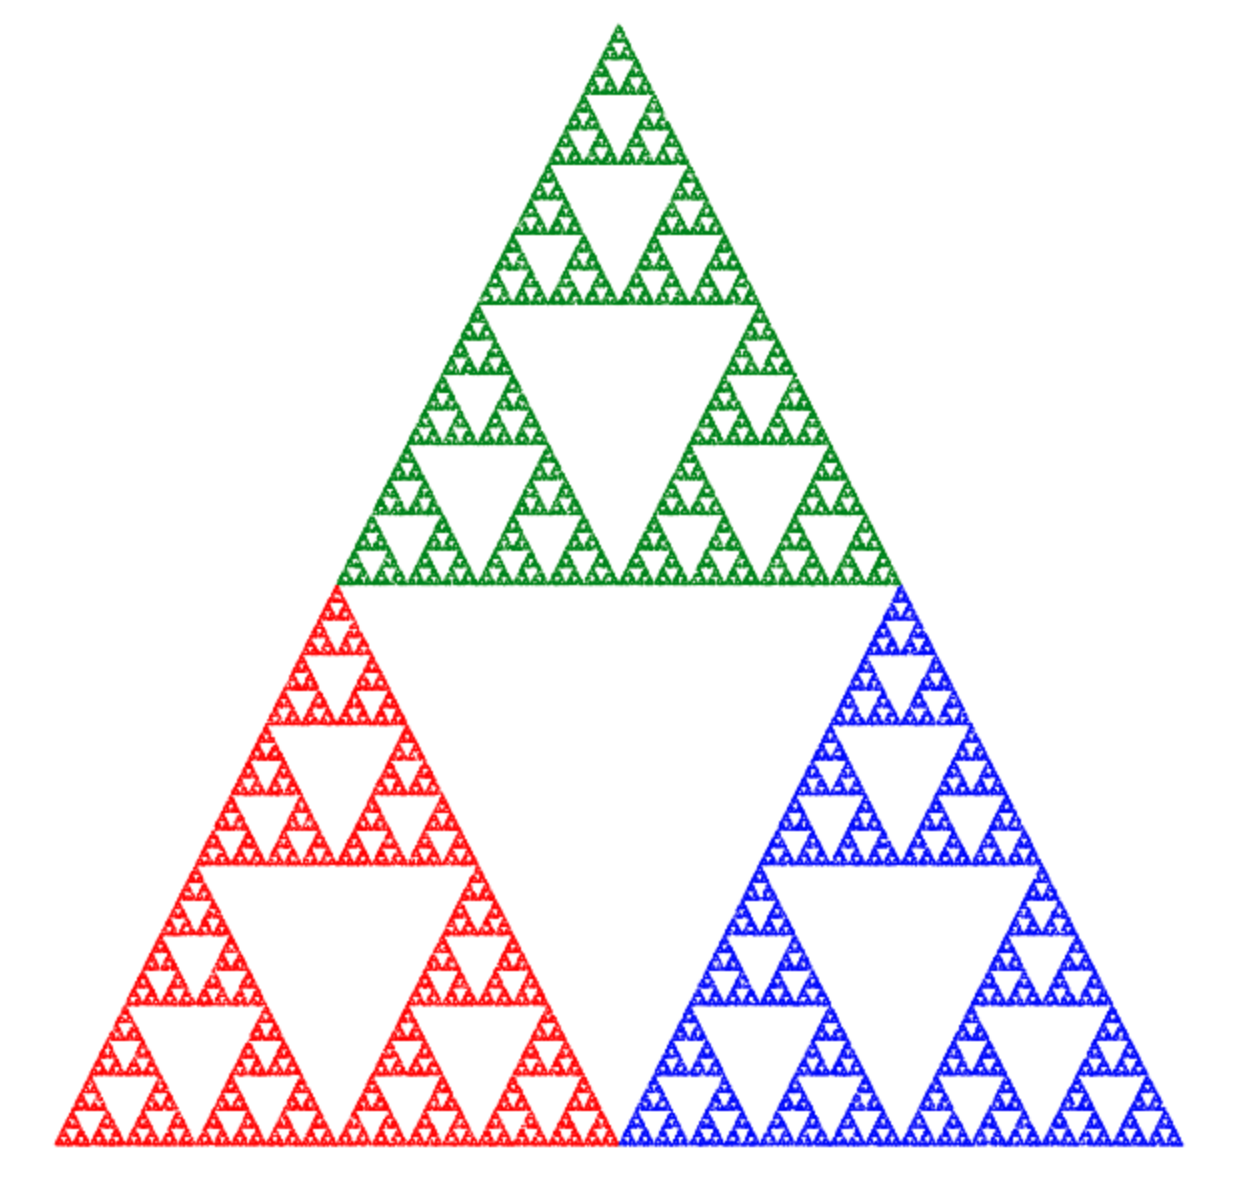
\includegraphics[width=8cm, height=8cm]{pic8.png}
       \captionof{figure}{3 Similar Clusters}
   \end{minipage}


\begin{algorithm}[1]
\caption{Generate IFS from Image}
\begin{algorithmic}[1]
\REQUIRE image\_path, n\_clusters = 3, iterations = 10000
\ENSURE IFS Points and Contraction Mappings
\STATE Load image from image\_path
\STATE Convert image to grayscale
\STATE Apply Otsu's thresholding to obtain binary image
\STATE Extract coordinates of non-zero points from binary image
\STATE Perform KMeans clustering on points to find cluster centers and labels
\STATE Initialize empty list for contraction mappings
\FOR{each cluster}
    \STATE Extract points belonging to current cluster
    \STATE Compute minimum and maximum coordinates of the cluster points
    \STATE Calculate scale factors:
    \STATE \hspace{1em} scale\_x = (max\_coords[1] - min\_coords[1]) / image\_width
    \STATE \hspace{1em} scale\_y = (max\_coords[0] - min\_coords[0]) / image\_height
    \STATE Ensure scale factors are within limits:
    \STATE \hspace{1em} scale\_x = min(scale\_x, 0.5)
    \STATE \hspace{1em} scale\_y = min(scale\_y, 0.5)
    \STATE Compute translation factors:
    \STATE \hspace{1em} translate\_x = min\_coords[1] / image\_width
    \STATE \hspace{1em} translate\_y = min\_coords[0] / image\_height
    \STATE Append (scale\_x, scale\_y, translate\_x, translate\_y) to mappings
\ENDFOR
\STATE Initialize points array for IFS
\STATE Set the first point randomly
\FOR{each iteration from 1 to iterations}
    \STATE Randomly select a transformation from mappings
    \STATE Apply transformation to the previous point to get the new point
    \STATE Append new point to points array
\ENDFOR
\STATE Plot the generated points
\STATE Print the contraction mappings

\end{algorithmic}
\end{algorithm}

This programme below takes the three pre-defined clusters shown above, and calculates the translation and scaling of each cluster using their minimum and maximum co-ordinates. Generating the IFS to be:

Transformation 1 $=\begin{bmatrix} 0.4645161290322581 &0\\0&0.5\end{bmatrix}\begin{bmatrix} x\\y \end{bmatrix} + \begin{bmatrix}0.267741935483871\\0\end{bmatrix}$
\\
\\
Transformation 2 $=\begin{bmatrix} 0.45483870967741935 &0\\0&0.4317111459968603\end{bmatrix}\begin{bmatrix} x\\y \end{bmatrix} + \begin{bmatrix}0.044623655913978495\\0.5248560962846677\end{bmatrix}$
\\
\\
Transformation 3 $=\begin{bmatrix} 0.45483870967741935 &0\\0&0.4317111459968603\end{bmatrix}\begin{bmatrix} x\\y \end{bmatrix} + \begin{bmatrix}0.5\\0.5248560962846677\end{bmatrix}$

This result doesn't look exactly like the IFS we were hoping to find, but by using the chaos game with these three transformations, we can find the image produced by this IFS.

\begin{minipage}{0.45\textwidth}
       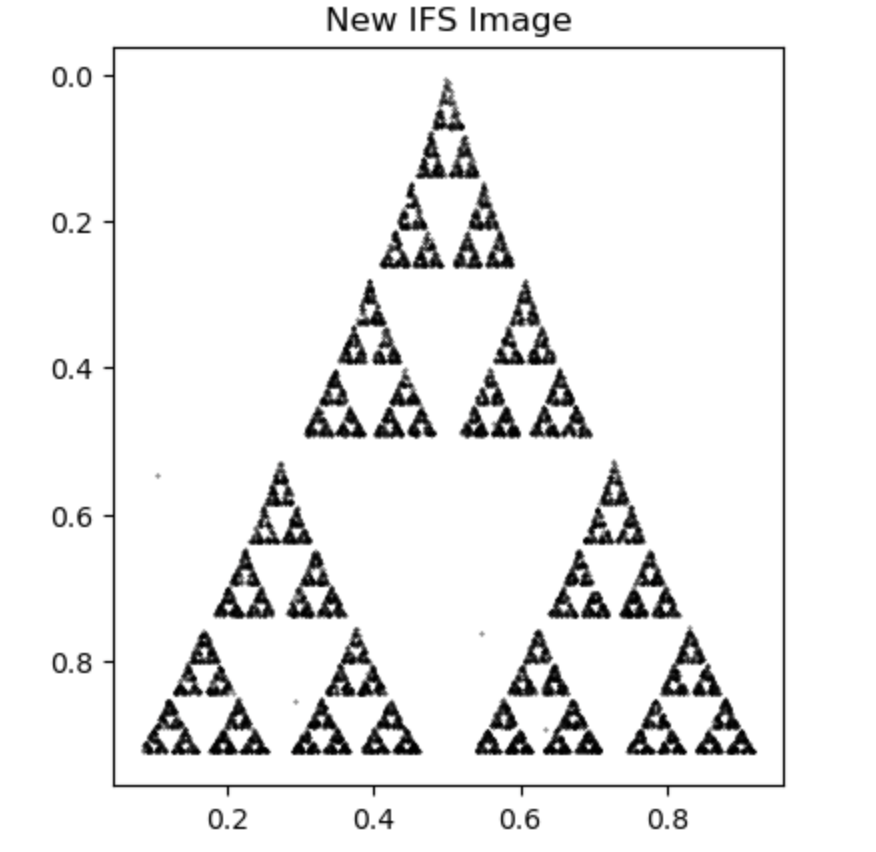
\includegraphics[width=10cm, height=10cm]{pic10.png}
   \end{minipage}
   \hfill
   \begin{minipage}{0.43\textwidth}
       This resulting image is visually very close to what we were hoping to achieve. However, each part of the is disconnected, due to the k-means clustering method. As well as this, there are many assumptions we have made in this model, thus many limitations.
    \end{minipage}
    \begin{itemize}
        \item The main assumption made was the fact that the image can be broken down into similar shapes due to the points being equal distance from each centroid. However, if we were to look at the Barnsley Fern fractal and implement the programme it would not work.
        \item We have also assumed that the transformations only consist of scaling and translation, when in reality there could be rotations and shearing.
        \item We have also penalised the scaling of x and y to take the minimum out of either the calculated scaling or 0.5, this forced their to be a contraction, but also limited the contraction to be less than 0.5 due to previous knowledge.
    \end{itemize}

   Overall this idea and method was influenced heavily by prior knowledge of what we wanted to find. Though our outcome was close to our goal this method is not really adaptable for other fractals and images, leading to our second idea.

   \subsubsection{Gradient Descent Optimization}
   This method doesn't use clustering, but instead gradient descent.This is an optimization algorithm used in machine learning which works to minimize the cost function of the model, where the cost function defines the difference between the predicted and true values to measure how well the model fits. The algorithm iteratively computes the gradient, which is the derivative of the cost function with respect to each parameter of the function, this tells us the direction of steepest ascent. Thus, by taking small steps in the opposite direction we move towards the minimum, this process repeats until the function converges to a minimum indicating the optimal set of parameters for the model has been reached.\cite{vidhya2020gradientdescent} 

   This method takes on a more brute force approach to the problem, where we have decided to initialize random affine transformations, for which we will use a gradient descent algorithm to optimize. 


\begin{algorithm}[1]
\KwIn{image\_path, num\_transformations = 3, max\_iterations = 1000, pixel\_subset\_ratio = 0.5}
\KwOut{Optimized affine transformation matrices, transformed image}

\textbf{Function:}read\_and\_process\_image(image\_path,scale\_percent):
\begin{algorithmic}[1]
\STATE Load image in grayscale
\STATE Resize image by scale\_percent
\STATE Convert resized image to binary using thresholding
\STATE \textbf{return} binary\_image
\end{algorithmic}

\textbf{Function:}extract\_black\_pixels(binary\_image):
\begin{algorithmic}[1]
\STATE Extract coordinates of black pixels from binary\_image
\STATE \textbf{return} black\_pixels
\end{algorithmic}

\textbf{Function:}plot\_image(pixels, title):
\begin{algorithmic}[1]
\STATE Plot pixels as scatter plot with inverted y-axis
\end{algorithmic}

\textbf{Function:}random\_affine\_transformations(num\_transformations,width, height):
\begin{algorithmic}[1]
\STATE Initialize empty list for transformations
\FOR{each transformation}
    \STATE Generate random scale and rotation matrix
    \STATE Generate random translation vector
    \STATE Combine into affine transformation matrix
    \STATE Append matrix to list
\ENDFOR
\STATE \textbf{return} transformations
\end{algorithmic}

\textbf{Function:}apply\_affine\_transformations(pixels,transformations):
\begin{algorithmic}[1]
\STATE Convert pixels to homogeneous coordinates
\STATE Initialize empty list for transformed pixels
\FOR{each transformation matrix}
    \STATE Apply transformation to pixels
    \STATE Append transformed pixels to list
\ENDFOR
\STATE Combine all transformed pixels into one array
\STATE \textbf{return} all\_transformed\_pixels
\end{algorithmic}

\textbf{Function:}chamfer\_distance(target\_pixels,transformed\_pixels):
\begin{algorithmic}[1]
\STATE Compute nearest neighbor distances from target to transformed pixels
\STATE Compute nearest neighbor distances from transformed to target pixels
\STATE Calculate mean Chamfer distance
\STATE \textbf{return} mean\_distance
\end{algorithmic}
\end{algorithm}

\begin{algorithm}
\textbf{Function:}loss\_function(transformation\_params,target\_pixels,num\_transformations, width, height):
\begin{algorithmic}[1]
\STATE Reshape transformation\_params into matrices
\STATE Apply transformations to target pixels
\STATE Compute Chamfer distance
\STATE Compute translation penalty
\STATE Compute scaling penalty
\STATE Compute eigenvalue penalty
\STATE Calculate total loss
\STATE \textbf{return} total\_loss
\end{algorithmic}

\textbf{Function:}optimize\_transformations(target\_pixels,width, height, num\_transformations, max\_iterations):
\begin{algorithmic}[1]
\STATE Generate initial random transformation parameters
\STATE Optimize transformation parameters to minimize loss function
\STATE Reshape optimized parameters into matrices
\STATE \textbf{return} optimized\_matrices
\end{algorithmic}

\textbf{Function:}main(image\_path,num\_transformations,max\_iterations, pixel\_subset\_ratio):
\begin{algorithmic}[1]
\STATE Read and process image to get binary image
\STATE Extract black pixels from binary image
\STATE Select subset of black pixels
\STATE Plot target image
\STATE Get image dimensions
\STATE Optimize transformation matrices
\STATE Apply optimized transformations to subset of pixels
\STATE Plot transformed image
\STATE Print optimized transformation matrices
\end{algorithmic}

\textbf{Main Execution:}
\begin{algorithmic}[1]
\STATE Set image\_path
\STATE Call main function with image\_path,num\_transformations, max\_iterations
\end{algorithmic}

\end{algorithm}

We focused on the same image of the Sierpinski Triangle that we had generated previously once again. The main steps of the algorithm are outlined here:
\begin{itemize}
    \item Converted our generated image into greyscale, this simplified the image into black and white pixels allowing us to extract the black ones and plot our ‘target image’. This image would represent the true values we use to calculate the cost function for out optimization.(In this case we have called it the loss function).
    \item Initialized a random affine transformation, where we have drawn randomn values from the normal distribution (mean 0.5, standard deviation $\sqrt{3})$ for the scaling and rotation. Then random values within the image’s dimensions for the translation vector, and combined to form a transformation matrix. 
    \item Take a subset of the black pixels and apply the initialized transformations to these points. 
    \item Calculate the chamfer distance between the target image points and the new generated points, so we can then determine the loss function that will be used to optimize our transformations for our chosen method. We chose to use the Chamfer metric instead of Hausdorff due to it being less sensitive to outliers, as stated in section 2 of this report.  
    
\end{itemize}

In an effort to obtain the desired IFS of the Sierpinski Triangle we implemented a few penalties to constrict the results to the loss function. 
\begin{itemize}
    \item The first penalty  penalizes the 2x2 submatrix, which represents the linear part of the affine transformation, including scaling, rotation, and shear components, having eigenvalues with absolute value > 1. This forces them to be contracting. 
    \item The second penalty is for large translations, by summing the boolean values that indicate large translations for each instance where a translation component exceeds the image bounds it is penalized. Maintaining the structural integrity of the transformed points, by encouraging the algorithm to find transformations that keep the translations within reasonable limits. 
    \item The third penalty penalizes non-uniform scaling by calculating the absolute difference between each eigenvalue (the same 2x2 submatrix as the first penalty) and 0.5, this comparison checks if the absolute deviation of any eigenvalue from 0.5 exceeds 0.1. 
\end{itemize}
Another focus was how to reduce the time it would take to run the programme, as computing the nearest neighbours each time is expensive. To combat this we instead extracted a subset of 50\% of the black pixels and changed the subset of black pixels used each time. 


Implementing this programme to our previously generated Sierpinski Triangle we obtained the transformations below and implemented them into a chaos game to visualise the IFS system:
Transformation 1=
\begin{bmatrix}
 -0.44917782 & 1.05575458 \\
  0.29773274 & -0.42933706 
\end{bmatrix}
\begin{bmatrix}
 x \\
 y 
\end{bmatrix}
+ 
\begin{bmatrix}
 148.13170073 \\
 99.13545204
\end{bmatrix}


Transformation 2=
\begin{bmatrix}
 0.404205507 & -0.740427725 \\
 -0.484694894 & -0.136360736
\end{bmatrix}
\begin{bmatrix}
 x \\
 y 
\end{bmatrix}
+ 
\begin{bmatrix}
 288.098280 \\
 319.656519
\end{bmatrix}


Transformation 3=
\begin{bmatrix}
 -0.52504087 & 1.18409974 \\
 -0.40187305 & 0.30264717 
\end{bmatrix}
\begin{bmatrix}
 x \\
 y 
\end{bmatrix}
+ 
\begin{bmatrix}
 127.14830966 \\
 294.30682285
\end{bmatrix}

\begin{minipage}{0.45\textwidth}
       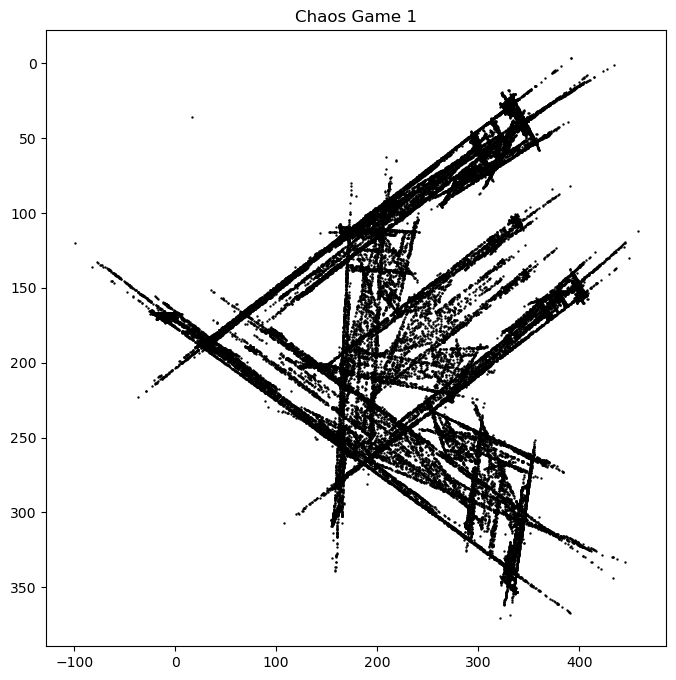
\includegraphics[width=8cm, height=8cm]{Chaos 1.png}
       \captionof{figure}{Transformation above}
   \end{minipage}
   \hfill
   \begin{minipage}{0.45\textwidth}
       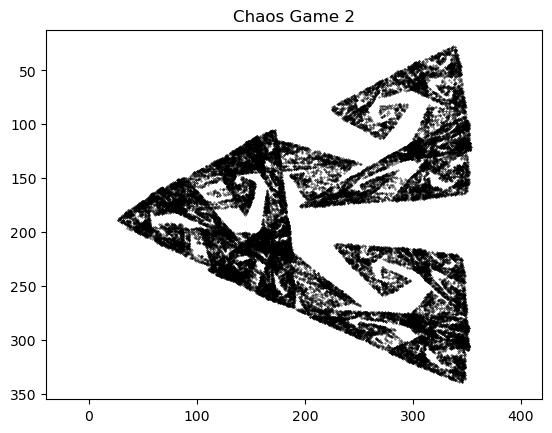
\includegraphics[width=8cm, height=8cm]{Chaos 2.png}
       \captionof{figure}{Transformations Below}
   \end{minipage}

Transformation 1= \begin{bmatrix} -0.479135509 & 1.00639798 \\ -0.41431358 & 0.0956091648 \end{bmatrix} \begin{bmatrix} x \\ y \end{bmatrix} + \begin{bmatrix} 167.993596 \\ 332.249866 \end{bmatrix}


Transformation 2= \begin{bmatrix} -0.279972639 & 0.47253439 \\ -0.392482158 & -0.260038796 \end{bmatrix} \begin{bmatrix} x \\ y \end{bmatrix} + \begin{bmatrix} 108.483713 \\ 328.812961 \end{bmatrix}


Transformation 3= \begin{bmatrix} -0.501802004 & 0.989770197 \\ -0.194601568 & -0.489740938 \end{bmatrix} \begin{bmatrix} x \\ y \end{bmatrix} + \begin{bmatrix} 176.340117 \\ 260.777769 \end{bmatrix}

We ran the test multiple times and unfortunately, the resulting images weren't exactly what we were hoping for. However, there are clear patterns and distinct triangle shapes similar to that of the Sierpinski triangle. Thus with further work on the code the Inverse IFS problem could be tackled with this method, for example our next step would be to try different metrics, or attempting to form our own.

\section{Conclusion}
The overall goal of this project was to formulate a way to convert an image into an IFS, for greater efficiency of image storage, to tackle the inverse IFS problem. The next step for this project would be to revise the algorithm for possible improvements towards time efficiency and accuracy, by altering the metric to compare points, then to implement this on other fractals we have generated throughout this report. This would put into perspective how adaptable the algorithm is and give a clear picture on how we could move forward.
The end goal would be to take any image, not just user generated fractals, and calculate an IFS that would create a similar image to closely approximate the original.







\newpage
%%%%%%%%%%%%%%%%%%%%%%%%%%%%%%%%%%%%%
% Acknowledgements
%%%%%%%%%%%%%%%%%%%%%%%%%%%%%%%%%%%%%
\section*{Acknowledgments}
%%%%%%%%%%%%%%%%%%%%%%%%%%%%%%%%%%%%%

\addcontentsline{toc}{section}{Acknowledgement}
First, we would like to thank our supervisor, Professor Lamb, for the inspiration and guidance into exploring the field of fractal image compression. His views and style of learning mathematics has motivated us to put our utmost effort into the project, despite the great difficulties we had in the beginning of this challenge.

We are particularly grateful to Professor Lamb's PHD student, Emilia Gibson, who aided us within the machine learning aspect of our project, giving us ideas to solve issues related to our gradient descent code. Some of our images that were generated would not have been as accurate and appealing, if it weren't for her.

Finally, we give acknowledgement to our ex-group member, Rongzhi Zhu, who had supported us within the theoretical part of the project, before he unfortunately left.

%%%%%%%%%%%%%%%%%%%%%%%%%%%%%%%%%%%%%

\nocite{*}
\bibliographystyle{plain}
\bibliography{ref}
%%%%%%%%%%%%%%%%%%%%%%%%%%%%%%%%%%%%%

\end{document}